
\documentclass[12pt,a4paper,english]{article}
\usepackage{graphicx, csquotes, babel, multicol, multirow, amssymb, fullpage, amsmath, tabularx, caption}
\usepackage[utf8]{inputenc}
\inputencoding{utf8}
\usepackage[T2A]{fontenc}
\usepackage[table]{xcolor}
\MakeOuterQuote{"}
\begin{document}

\title{Analysis of knowledge requirements for speech and text alignment problem}
\author{Bartosz Kalińczuk}
\date{\today}
\maketitle

\newpage
\begin{abstract}
The purpose of this final master degree project was to experiment with various algorithms for speech and text alignment either with granularity of sentences, single words or even single phonemes. The output of this study was expected to find out how little data is necessary to compute a proper alignment. This project focuses mainly on Polish language, however it can be quite easily generalized for different languages. It also focuses solely on a audio with quite low level of noise, since noisy environment introduces a lot of problems, and is out of the scope of this project.
\end{abstract}


\newpage
\setcounter{tocdepth}{2}
\tableofcontents

\newpage
\section{Introduction}

The purpose of this final master degree project was to experiment with various algorithms for speech and text alignment either with granularity of sentences, single words or even single phonemes. The output of this study was expected to find out how little data is necessary to compute a proper alignment. This project focuses mainly on Polish language, however it can be quite easily generalized for different languages. It also focuses solely on a audio with quite low level of noise, since noisy environment introduces a lot of problems, and is out of the scope of this project. \newline

In two first chapters I would like to present a theory behind speech signal processing and speech recognition,
that is well known and understood, and is mentioned in many different papers regarding speech related problems. I also introduced here a frontend part of Sphinx library, which implements a popular way of speech signal preprocessing, which I reuse in this project. \newline

The chapter 4 is exploring a simple approach with minimal knowledge, that produces very crude results. The minum knowledge here is enough reason to bring it up, but I also found some another application for this imperfect solution. \newline

Next two chapters are exploring a possibility of using audio models from foreign languages to achieve alignment with satisfying accuracy.
The keynote of this part of thesis is a study of similarities between languages and their phonetics. I present here not only my own algorithms, but also certain parts of sphinx library, which I used: including tool for alignment problem using preprocessed audio model and dictionary, and in other case only state scorers from trained English and Russian models. \newline

The chapter 7 combines conclusions and knowledge of previous chapters to study what can be done without any trained models and what knowledge is enough to align text for practical applications. \newline

In the end I'm trying to show a small application of all presented solutions and show the results in more practical manner. \newline

I try to approach this topic with a hackish scientific curiosity. The problem is presented, but I try to check what can be done if I redefine it in various configurations. I don't focus purely on results, because they are not as interesting as exploration of the area just to see what is there. \newline

\newpage
\begin{center}
    \section{Speech signal}
\end {center}
\subsection{Human factor}

Speech is a most efficient way the human communicate. For generations this process was refined by evolution, so we can easily exchange messages even in noisy environment. For this purpose our vocal mechanisms must well cooperate with our hearing ability. There is a certain set of sounds we can produce and our ears evolved to hear them as well as possible.\newline 

What is sound? According to dictionary: "Vibrations transmitted through an elastic solid or liquid or gas, with frequencies in the approximate range of 20 to 20000 hertz, capable of being detected by human organs of hearing". [1]\newline

How do we hear? Human ear consist about 30000 hair-cells, which can convert mechanical wave of the sound into electromagnetic wave inside auditory nerves [2]. 
Each of these cells is excited by different frequency of mechanical wave of internal ear fluids, so it is no surprise, that people can hear only a certain range of frequencies, as stated in definition. These we expect to be finely tuned to the range of the sounds we can produce. Although it seems, that we can hear a bit more, but as we don't need that, it happens, that as we grow older, our hearing range is getting smaller, because our hearing cells fail sometimes, but mostly those responsible for high frequencies, which we don't use too often.\newline

Humans can hear frequencies, that begins as low as 12Hz (under laboratory conditions) to 20kHz (for adults usually much lower). However speech range is a little bit smaller than that [3]: \newline

\begin{figure}[hb]
    \centering
    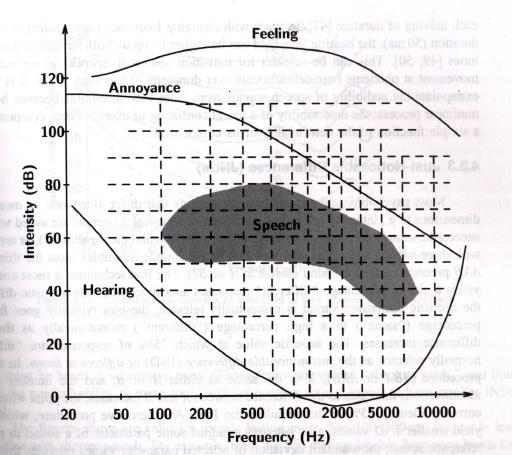
\includegraphics[scale=0.5]{speech_range.jpg}
    \caption[]{Speech range from [3] \emph{Fundamentals of speech recognition}}
\end{figure}


\newpage
\subsection{Mel scale}

How we perceive sound, that is completely different matter and topic for long philosophical discussion. However we can help ourselves with some subjective experiments. For example Stevens, Volkman and Newman conducted an experiment on a number of listeners to measure, what do we perceive as equally distanced pitches. In this experiment, the participants of the experiment were asked to judge if given pitches were in equal distances. The output was, that humans don't experience sound linearly respectively to the frequency scale, but a perceptual scale was closer to logarithmic one. [5] \newline

Certain formulas were conceived to translate frequency scale to one, that is closer to how human actually perceive sound. \newline

One popular is mel scale, where mel comes from melody: [6] \newline
\begin{equation}
    m = 2595 \: \: log_{10}(1 + \frac{f}{700})
\end{equation}
where $f$ is a frequency and $m$ is scaled melody frequency. \newline
This looks as in the plot:
\begin{figure}[hb]
    \centering
    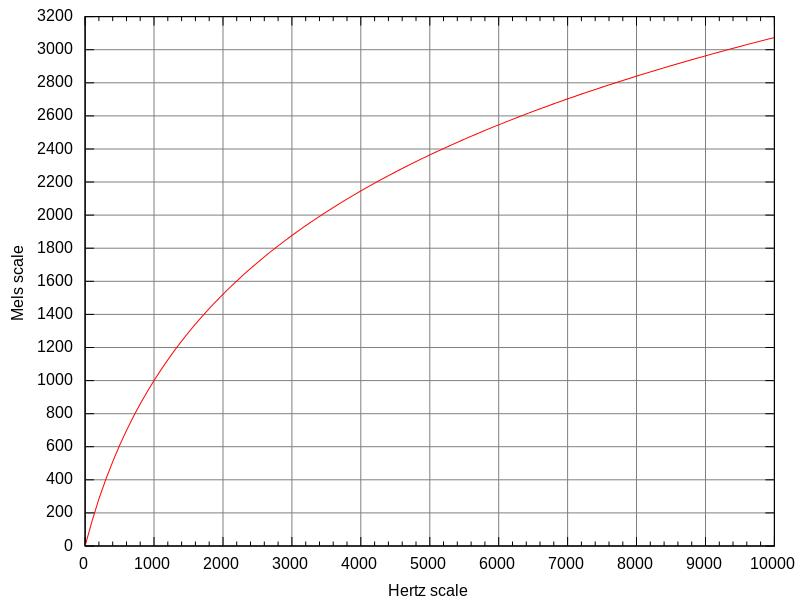
\includegraphics[scale=0.3]{mel_scale.jpg}
    \caption[]{Mel scale from http://en.wikipedia.org/wiki/Mel\_scale}
\end{figure}

Another popular formula of so called bark scale, which is based on perception of loudness of the sound and proposed by Eberhard Zwicker in 1961. [7] \newline
\begin{equation}
    Bark = 13 \: \: atan(\frac{0.76f}{1000}) + 3.5 \: \: atan(\frac{f^2}{7500^2})
\end{equation}
In this project we use mel scale implemented in sphinx library, although bark scale is becoming more popular recently.

\newpage
\subsection{Frequency spectrum}

The conclusion from the anatomy of human ear is, that frequencies of the sound are important.
How can we obtain frequency spectrum from a digitized sound, so we can proceed further? \newline
The obvious tool for conversion of discrete function to frequencies is Discrete Fourier Transform, named after Jean Baptiste Joseph Fourier it is one of the most often used techniques of modern times. \newline

It all started from the postulate, that a heat equation can be satisfied by function of form: [11] \newline
\begin{equation}
    f(x)=\sum_{n=0}^N(A_n cos(nx) + B_n sin(nx))
\end{equation}
or in complex form:
\begin{equation}
    f(\theta)=\sum_{n=-\infty}^{\infty} C_n e^{i n \theta}
\end{equation}

Basically we convert our function's domain to frequency domain or to domain of sinusoidal functions. $C_n$ coefficients are complex values that encode both amplitude and phase of the converted signal/function at each frequency. \newline

The coefficients for any integrable functions over an interval $[\frac{-T}{2}, \frac{T}{2}]$ can be obtain using formula: [11] \newline
\begin{equation}
    C_n=\int_{\frac{-T}{2}}^{\frac{T}{2}} f(x) e^{-2 \pi i \frac{n}{T} x} dx
\end{equation}

or for the discrete case:
\begin{equation}
    C_k=\sum_{n=0}^{N-1} x_n e^{\frac{-2 \pi i k n}{N}} dx
\end{equation}
	

So far we haven't found any use in the speech recognition for phase part of the coefficients, however amplitude determines how powerful is signal at given frequency. The power value is given by ($X_k$ is a complex coefficient):
\begin{equation}
    |X_k|/N = \sqrt{\Re e(X_k)^2 + \Im m(X_k)^2} / N
\end{equation}

\newpage
A sample conversion:
\begin{figure}[hb]
    \centering
    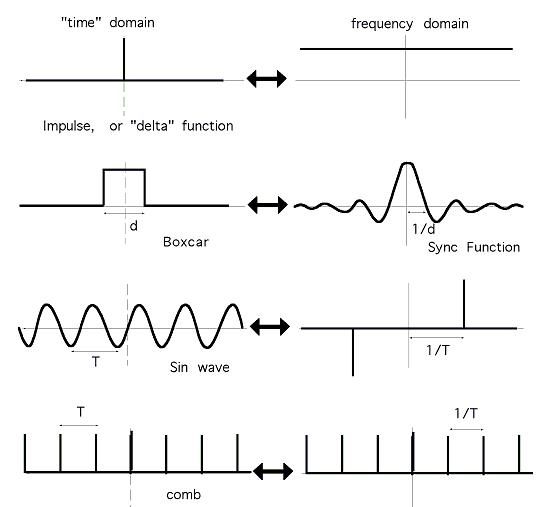
\includegraphics[scale=0.3]{sample_dft_conversion.jpg}
    \caption[]{Example of Discrete Fourier Transform from brokensymmetry.typepad.com}
\end{figure}

What size of the window should we use? First we have to notice, that in order to capture certain frequency, the window needs to be large enough. We would like to examine signals of frequency ranged from 100Hz (see speech frequencies ranges in chapter 2.1), which is a period of 100th of the second, so a 10millisecond window would be our bottom limit. \newline

Also windows with abrupt signal discontinuities may cause result with spectral artefacts, so a windowing function is usually applied. Popular choice is a Hamming window function: [8]
\begin{equation}
   w_j = 0.54 - 0.46 cos(\frac{2 \pi j}{W - 1}) 
\end{equation}
where $W$ is a window size (number of frames) and $j$ is a frame number and resultin $w_j$ is scaling weight.
The function's plot is given below:
\begin{figure}[hb]
    \centering
    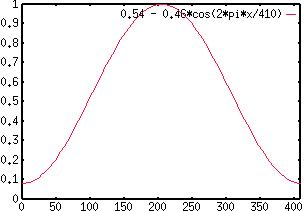
\includegraphics[scale=0.5]{hamming_window.jpg}
    \caption[]{Hamming window example from sphinx4 javadoc}
\end{figure}

\newpage
Note that it emphasises values in the middle of the window, so our actual windows should overlap to cover whole time domain. For example by shifting a window by a percentage of it actual width:
\begin{figure}[hb]
    \centering
    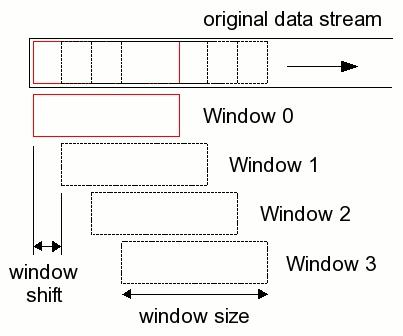
\includegraphics[scale=0.3]{window_shifting.jpg}
    \caption[]{Window shifting example from sphinx4 javadoc}
\end{figure}

A human speech signal in frequency and time domain plot, which shows powers of signal at each frequency: [3]
\begin{figure}[hb]
    \centering
    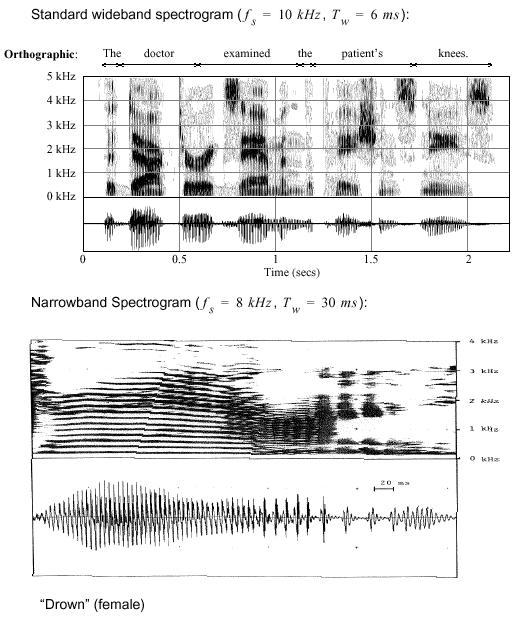
\includegraphics[scale=0.5]{speech_spectrogram.jpg}
    \caption[]{Example speech signal from [3] \emph{Fundamentals of speech recognition}}
\end{figure}

\newpage
\subsection{Cepstrum}

Looking at the frequency spectrum of human speech we see, that  the signal in the frequency domain contain features that are quite periodic. As it is with converting initial signal with DFT, we would like to extract the information of periodicity in the spectrum. 
A cepstrum of the signal gives us this additional information. \newline

The word is derived by reordering characters in the word spectrum to indicate switch of domains, similarly as word 'quefrency'. The cepstrum operates in the domain of time and the basic intuition is, that it reveals a rate of change in the different spectrum bands. 
For example a cepstrum of an echoed signal in the picture below shows clearly a three 'quefrencies' of the echo of the signal. [12]
\begin{figure}[hb]
    \centering
    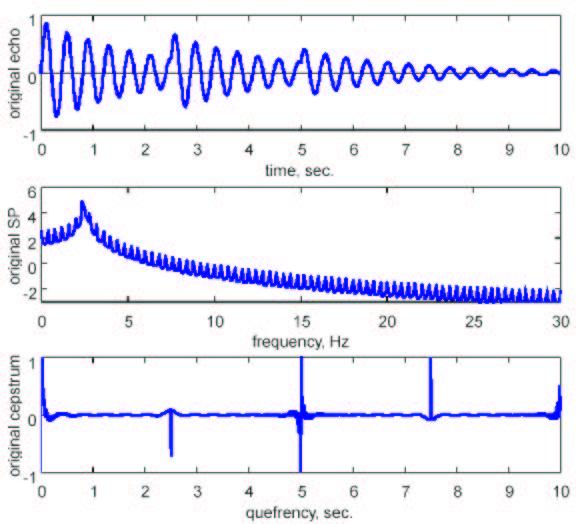
\includegraphics[scale=0.4]{echo_cepstrum.jpg}
    \caption[]{Cepstrum of signal with echo from [12] \emph{The Quefrency Alanysis of Time Series for Echoes}}
\end{figure}


Cepstrum definition is: "Inverse Fourier transform of the logarithm of the magnitude of the Fourier transform" or:
\begin{equation}
    C=|F^{-1}{log(|F{f(t)}|^2)}|^2
\end{equation}

or:
\begin{equation}
    c_x[n] = \frac{1}{2\pi} \int_{-\pi}^{\pi}log |X(e^{j \omega})| e^{j \omega n} d\omega
\end{equation}

This is the definition of the power cepstrum, since it is calculated from the magnitude of each frequency band. However there also exists a complex, real and phase cepstrum depending on what part of initial Fourier transform it uses.
In speech related problems a power cepstrum is usually used and I haven't see any reason to not focus only on this.


\newpage
\addtolength{\textwidth}{6cm}

\begin{minipage}[-200,0]{5cm}
    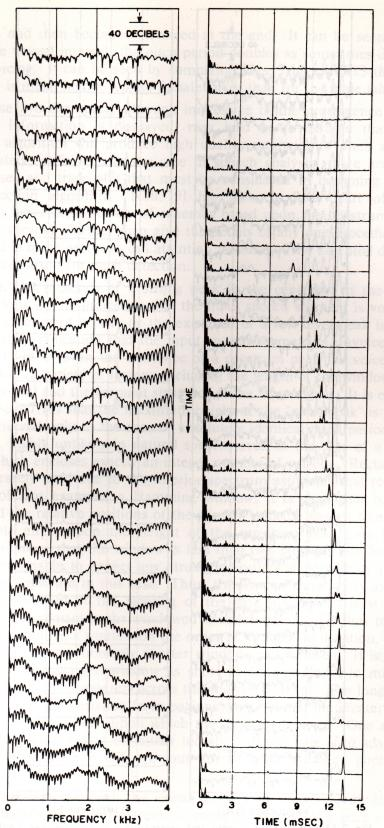
\includegraphics[width=5cm,height=20cm]{vowel_cepstrum.jpg}
\end{minipage}
\begin{minipage}[5cm,0]{11cm}

If the sound becomes periodic in the frequency domain it's quefrency domain contains a peak which is related to the periodicity of the sound. \newline

Note that similar results can be obtained by taking just additional DFT of the signal. Inverse Fourier Transform is closely related to Fourier Transform and also performs a split of the function into periodic components. \newline
\newline
After all IFT is defined:
\begin{equation}
     f(x) = \int_{\mathbb{R} ^ n} e^{2 i \pi x \zeta} \hat{f}(\zeta) d\zeta
\end{equation}
while FT is defined: 
\begin{equation}
    \hat{f}(\zeta) = \int_{\mathbb{R} ^ n} f(x) e^{-2 i \pi \zeta x} dx
\end{equation}

Why taking logarithm of the magnitude? It serves as a normalization of power spectrum. In speech for example it happens, that low frequency components are usually more powerful than high frequncy components and by normalizing the signal, the periodicity becomes more apparent. \newline


A bit different way of looking at the signal cepstrum is as a homomorphic transformation which changes convolution into sum. [3]
\begin{equation}
x(n) = e(n) * h(n)
\end{equation}
\begin{equation}
\hat x(n) = \hat e(n) + \hat h(n)
\end{equation}


Which on it's own can be seen as way of separating signals, since it is more easy to extract elements from a sum, than from a convolution.
\newline
\newline
In the example with echo (fig.7) a cepstrum of signal have clear peaks, which indicate repetitions of initial signal. Conversion the initial convolution of frequency spectrum to sum of signals in a cepstrum form, allows us to separate echoed signal from original signal, and it might also be used to filter out an audio feedback.

\end{minipage}
\newline
\newline
\captionof{figure}{This is a typical cepstrum sequence of the vowel computed every 10ms taken from [3] \emph{Fundamentals of speech recognition}}
\label{fig:fig1}

\newpage
\subsection{Sphinx frontend}


Sphinx is a speech recognition toolkit with a lot of useful functionalities for any speech related problem.  \newline
The main feature of Sphinx library is a speech recognition using input audio model and dictionary. However it is a modular and open source library,
so it is easy to use any part inside different projects, like signal preprocessing (fronted part). In addtion there are some example tools, that can be used separately, like
for example audio model based aligner. \newline

There is a certain common way to prepare a speech signal for the further processing. With slight variations in each step, the useful informations about speech are drawn from a cepstrum of the reduced signal (in the number of data dimensions), as presented in this chapter. \newline

In order to skip the reinvention of the wheel, I used the fronted part of the sphinx library in any experiment in this project.
The sphinx fronted performs signal transformation and produces data composed of only 39 voice features,
while actually only 13 are base ones and the rest is a derivation of these, what is also quite common choice among speech related projects. \newline

Sphinx frontend is a list of transformations executed on the result of the transformation placed higher in the list.
In another words it is a transformation composition. \newline
\newline
This Sphinx frontend pipeline includes: \newline
\begin{itemize}
	\item Data Blocker,
	\item Preemphasizer,
	\item Windower,
	\item Discrete Fourier Transform,
	\item Mel Frequency Filter Bank,
	\item Discrete Cosine Transform,
	\item Cepstral Mean Normalization,
	\item Deltas Feature Extractor.
\end{itemize}
I'll try to introduce them a bit closer to show, how speech signal can be transformed to a useful form of small feature vectors.

\newpage

\subsubsection{Data Blocker}

This initial transformation reads incoming double data read from audio source (file or microphone) and
prepares blocks of the data to be used in later phases. In our case blocks contain 10ms of audio data.

\subsubsection{Preemphasizer}

The Preemphasizer applies a formula: $Y[i]=X[i]-(X[i-1] * preemphasizerFactor)$.
The purpose of this transformation is to emphasize the high frequency components. It is kind of filter,
which allows high frequency components to pass through, but weakens the low frequency ones.


\subsubsection{Raised cosine windower}

Creates windows from the incoming data. A windowing function
\begin{equation}
    W(n)=(1-\alpha) - \alpha cos(\frac{2 \pi n}{N - 1})
\end{equation}
 is applied afterwards. Alpha coefficient set to 0.46 results with a mentioned before Hamming windowing
 function, which is a default setting and the one used by me.

\subsubsection{Discrete Fourier Transform}

Sphinx performs this step using its own implementation of Fast Fourier Transform.
The FFT can perform transformation with complexity $\Omega(Nlog(N))$, where N is the size of the input data.
It can be perform on whole data, however in speech we would like to get an information of the frequencies 
of a small frame, that contains consistent speech signal, in particular a single phoneme.
The output data is the power spectrum of input data window and the complex/phase information is lost.
The number of FFT points is the closest power of 2 equal or larger to the number of samples in the incoming window of data. However the input signal is real, so resulting FFT is symmetric, so only half of the data is returned and the output size is $\frac{FFT points}{2} + 1$.

\newpage

\subsubsection{Mel frequency filter bank}

This step is a part of calculating a Mel Frequency Cepstrum. \newline

Conversion of frequency spectrum into a mel-spectrum using triangular overlapping windows defined as:
\begin{equation}
    w(n) = 1 - |\frac{n - (N - 1)/2}{(N + 1)/2}|
\end{equation}


The number of triangles/filters defined the size of mel-spectrum and the sphinx's default is 40. \newline
The filters are chosen, so the result would simulate a mel-scale given by the formula:
\begin{equation}
    melFreq = 2595 log(1 + linearFrequency / 700)
\end{equation}

The given filters should look like in the picture:
\begin{figure}[hb]
    \centering
    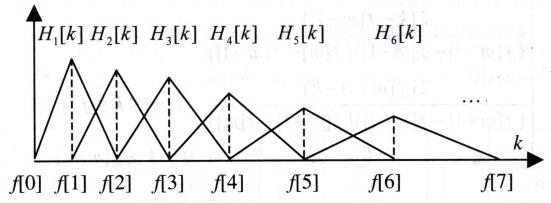
\includegraphics[scale=0.4]{mel_filters.jpg}
    \caption[]{Melody filters from [3] \emph{Fundamentals of speech recognition}}
\end{figure}

Not all frequencies are covered by the filters.
The chosen range of frequencies may differ for various audio encodings,
but generally should cover only the speech ranges.
The default values for 16kHz sample rate streams are 130Hz-6800Hz and are not changed in this project.

\subsubsection{Discrete Cosine Transform}

Another part of calculating Mel Frequency Cepstral Coefficient vector (MFCC).  \newline

It applies a logarithm and the DCT type II to the input data.  \newline

A DCT type II (most common) coefficients are defined as: 
\begin{equation}
    C(u) = \alpha(u)\sum_{x=0}^{N-1} f(x)cos[\frac{\pi(2x+1)u}{2N}] 
\end{equation}
and it is quite tightly related to real part of the Fourier Transform. [18]
The transform represents a function as a sum of cosine functions and it is equivalent to the DFT operating
real data with even symmetry. \newline
The number of dimensions returned is set by default to 13, what is quite common choice. The first feature is closely related
to energy of the speech signal (not completely, since IFT was performed only on magnitudes of frequencies coefficients).

\subsubsection{Cepstral Mean Normalization}

Performs a normalization of MFCC vector by subtracting a mean of all the input. There are two versions
of this step. One that calculates mean online and the other that reads all data before performing
subtraction.

\subsubsection{Deltas feature extractor}

The final transformation in the sphinx frontend chain. It calculates first and second order derivative of the
cepstrum as additional features of the speech signal. It improves noticeable speech processing algorithms
by adding additional information about changes in the cepstrum data. \newline

For the initial cepstrum data it adds additionally twice the size vector with first and second order
differences, calculated as shown in the picture:
\begin{figure}[hb]
    \centering
    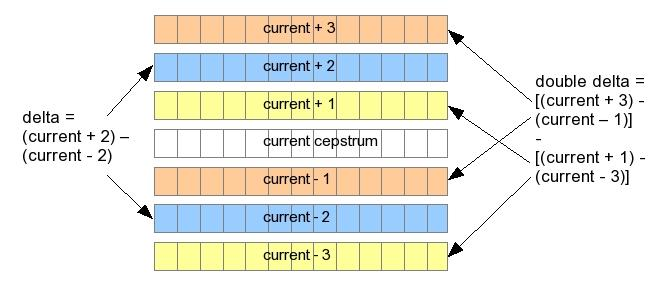
\includegraphics[scale=0.6]{deltas_calc.jpg}
    \caption[]{Deltas explanation from sphin4 javadoc}
\end{figure}

\newpage
\begin{center}
    \section{Speech Modelling}
\end {center}
\setcounter{equation}{0}

\subsection{Phones, phonemes and graphemes}

A phone is a unit of speech sound [20]. Phoneme's definition is: "The smallest contrastive linguistic unit, which may bring about a change of meaning" [21], so the phoneme is a classification unit of phones, which allow us to represent speech while preserving its meaning.  While speech is being modelled using phonemes the graphical part of the language in form of text is modelled with characters or graphemes. \newline

Language grapheme set usually differs from it audio counterparts, although it does depend on, which language are we talking about. English seems to differ quite a lot, while Italian not so much, what seems to be related to adoption of Latin alphabet. Polish grapheme and phoneme sets are quite similar, although there are some differences. Usually the grapheme set contains more characters than needed to represent every word from given language and at the same time it is much too small to represent all the nuances of human speech. What is more problematic, the word graphic representation sometimes has very little to do with actual phones of the word. I.e. there are so called homographes: words, that are written the same yet they pronunciation differs ("zamarzać" from "marznąć" and "morzyć") or homophones, that look differently, but are pronounced similar ("może", "morze"). In polish though, the former is quite rare and this fact is actually used by me (chapter 5.3). \newline


Actual phones that are classified under single phoneme create a diversified family.  Different variants of a phoneme are called allophones. For example /l/ in English "leap" and "deal" or polish examples of allophones (/ł/ in "umysł" might be soundless contrary to "ławka") or vowels between soft consonants (/a/ in "jajko"). [22] \newline

The phonemes can differ quite substantially depending on the surrounding phones. For example almost each phoneme in polish changes to softer version when put next to /i/ or /j/, although sometimes the change is so substantial, that we no longer talk about allophone, but a completely separate phoneme ('ć' $\iff$ 'c', in contrast to vowels' changes). Notice, that the choice of extracting allophone to a completely new phoneme is all about checking, if leaving it as it is, won't create a situation, where we are unable to distinguish two words with different meaning (see phoneme definition).
Additionally consecutive phones are not necessarily separated by clearly visible moment of silence. Often one phone is converting slowly into another. To model such a transitions a each middle phoneme of all triphones (sequence of three phonemes) are modelled seperately and stored with a context (neighborhood). \newline

Phonemes are very important in the computational language modelling, either in speech recognition or alignment. The importance is derived directly from its definition. It is a unit of speech, which can't be switched to another without changing the meaning. This is the unit, that need to be modelled if we want to recognize and/or distinguish different words. Finer granularity of model is necessary only to make a better prediction where an observed phone belongs.

\newpage
Some of English phonemes and example phones:
\begin{figure}[hb]
    \centering
    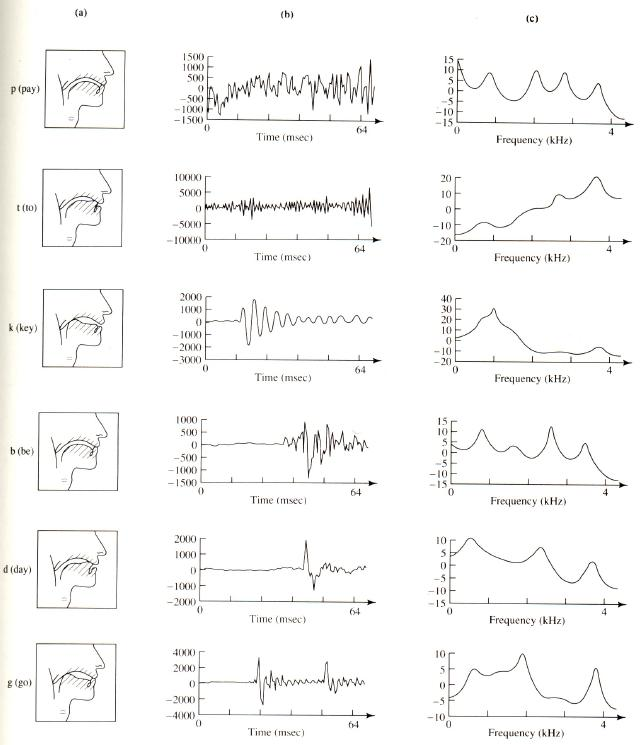
\includegraphics[height=8.7cm, width=13cm]{example_phones_1.jpg}
    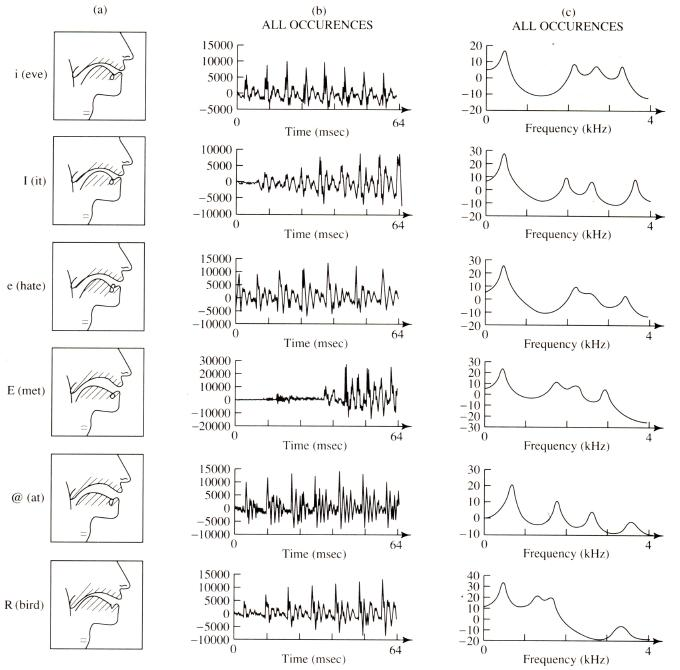
\includegraphics[height=8.7cm, width=13cm]{example_phones_2.jpg}
    \caption[]{Example phones from [3] \emph{Fundamentals of speech recognition}}
\end{figure}

\newpage
\subsection{Audio distances}

The simplest way to find similar audio sequence is to find a sequence which is nearby to another,
that we know represents a certain sound, phoneme or word. [16] \newline

To calculate a distance we could use various norms:
\begin{equation}
    ||x||_1 , || x ||_2, ... , || x ||_\infty
\end{equation}
, where 
\begin{equation}
    ||x||_k = (\sum_{i=0}^{N} x_i^k)^\frac{1}{k}
\end{equation}
and $x$ is a signal frame or its feature vector. \newline
All such norms are fine for uncorrelated vectors, which is really the case with speech signal. \newline


For correlated vectors, we could try to introduce some weighting factor inside.\newline
What factor should we use?\newline
One approach is to tune the factors using external methods, which theoretically may give us some additional benefit of properly modelling phonemes, that we try to measure distance from, however this is a bit out of the scope of this chapter and most probably would in the end look similar to a different method.
A simpler approach would be to calculate correlations and use them in a distance measure.
If we had a correlation matrix ($P$) and than our distance could be:
\begin{equation}
    dist_{using correlations}(\vec x, \vec p) = (\vec x - \vec p)^T P^{-1} (\vec x - \vec p)
\end{equation}
               
Karl Pearson introduced such an idea [23] in form of correlation coefficient defined between two random populations:  
\begin{equation}
    \rho_{XY} = \frac{cov(X, Y)}{\sigma_X \sigma_Y} = \frac{E[(X - \mu_X)(Y - \mu_Y)]}{\sigma_X \sigma_Y}
\end{equation}
where $\sigma_X$ is a variation of random variable $X$ and $\mu_x$ is its mean value. \newline
In matrix form:  
\begin{equation}
    P = (\Sigma^{diagonal})^{-1/2} \Sigma (\Sigma^{diagonal})^{-1/2}
\end{equation}
where $\Sigma$ is a covariance matrix and $\Sigma^{diagonal}$ is a diagonal matrix created from $\Sigma$,
so its non-zero entries are variances of random variables. \newline

It should be noted, that in the denominator we have standard deviations which don't really bring any value to our measure, since this is a constant factor.
By removing them we obtain so called Mahalanobis distance [16]:
\begin{equation}
    distance_{Mahalanobis}(\vec x, \vec p) = (\vec x - \vec p)^T \tilde C^{-1} (\vec x - \vec p)
\end{equation}

If we knew elements belonging to any given phoneme, we could calculate a distance between this training sample and any encountered speech signal.

\newpage
\newpage
\subsection{Experiments}

I conducted couple of experiments with different distances.
Starting with a flawed alignment of larger portions of text I tried to:
\begin{itemize}
	\item find the same word, that is quite lengthy and occurs multiple times just by searching for similar sequences,
	\item find a given sequence of three phonemes in a text, based on estimated location (time)
\end{itemize}
The idea behind these experiments, was to see if similarities in speech can be found based on similarities in text.
In theory if we could match similar sequences, than maybe we could derive from the matching a phoneme set (with example phones), that could be used in further studies. \newline
In both experiments different distance measures was used, to see how helpful they are at separating different phonemes. \newline

In first experiment I chose some long word, that occured more then once in the text. Then I'll estimated the times it should appear in the speech and then for quite large areas (which was more or less of $O(\sqrt{total \: \: time})$ in size) around the estimated time, I searched for the most similar sequences either with a speech signal in form of feature vectors described earlier as well as vector of frequency magnitudes. \newline
This experiment was an utter failure, since it always found two familiar sequences, that were in no way familiar in speech sense.
However I also tried to see how it behaved with marked one occurence of the word, and then it was actually able to find other occurences, ... sometimes. \newline

In the second experiment I picked first three letters of the text and a portion of detected speech, which suppose to be aligned together. I found all occurences of the letters and then I proceded in similar manner, as in first experiment. I estimated time they all should appear in recording and then I have tried to find them within a certain neighborhood of the estimated times. It wasn't a success, but I was able to find around 50\% of all occurences of three letter sequence from beginning of the text and other found were quite similar (80\% of the time they contained two out of three phonemes), although I was lucky, that in my testing recording, the starting three letter sequence occurrences in the text were quite far from each other, so I never searched twice the same area. \newline

My conclusion is, that the Euclidean norm were performing the best, although Mahalanobis distance in those experiments were not expected to give any significant results, since there were conducted without knowledge of phone classification and it behaved without a surprise. \newline

\newpage
\subsection{Gaussian Model}

Given observation points belonging to a single class (a phoneme) with a given probability,
we would like to model a distribution of emitting data point by the class. \newline


A natural choice is a normal distribution, although we have to remember, that observation comes from a multidimensional universum, where populations are not independent. \newline
Luckily there is a definition of multivariate normal distribution, that considers correlations:
\begin{equation}
    f_x(x_1,...,x_k) = \frac{1}{\sqrt{(2\pi)^k |{\Sigma}| }}exp(-\frac{1}{2}(x-\mu)^T{\Sigma}^{-1}(x-\mu))
\end{equation}
                       
where $\Sigma$ is a covariance matrix and $|\Sigma|$ is its determinant. \newline
The problem with this vector arises, when $\Sigma$ matrix is singular, which is not invertible nor it has determinant. This can happen quite often, when the observation data is too small. \newline

Covariance matrix is always symmetric and positive-semidefinitive.\newline
Symmetry comes directly from a definition: $cov(X) = E[(X - E(X))(X - E(X))^T]$, since outer product of a single vector gives always a symmetric matrix. \newline

Positive-semidefinitive matrix is a matrix, where for any product $a^T A a$ with any non-zero complex vector $a$ is real and non-negative:
\begin{equation}
    a^T A a >= 0
\end{equation}

A product with any vector $a$ and covariance matrix is also equal to: 
\begin{equation}
    a^T \Sigma a = a^T E(XX^T) a + a^T\mu\mu^T a = \frac 1 N (\sum_{i=1}^N a^T X X^T a) + a^T\mu\mu^T a
\end{equation}
and each element of the sum is square of inner product of two vectors, so it is always positive (or equal to zero). \newline

In order to prevent degenerate cases we can allow only positive-definite matrices. \newline
Any such a matrix is guaranteed to be invertible. \newline


If the number of dimensions is equal to one, then the formula reduces to single-variable normal distribution: 
\begin{equation}
    f(x) = \frac 1 {\sqrt{(2\pi)}\sigma}e^{-{ \frac {(x-\mu)^2}{2 \sigma^2}}}
\end{equation}


\newpage

A normal distribution of emitting signal frame have two free parameters: a mean vector and a covariance matrix,
which needs to be calculated.\newline
I assume, that an input is the list of observations with assigned probability.\newline 

If probability is actually a likelihood of emitting the signal (or its estimation),
than we can calculate mean with a formula:   
\begin{equation}
    \vec \mu = \sum_{\vec X} Pr(\vec X) \vec X
\end{equation}
and a covariance matrix by: 
\begin{equation}
    \hat C = \sum_{vec X} Pr(\vec X) (\vec X - \mu) (\vec X - \mu)^T
\end{equation}
\newline


In the case, that probability is not a direct likelihood of given point, but a conditional probability of emitting the signal,
(i.e. under the condition that it belongs to given sequence), the probabilities need to be normalized first. \newline

We can assume, that conditional probability is the same for each observation,
 so the input probability is in the form of $ Pr(\vec X) Pr_{condition}$,
then they have to be divided by a total sum to produce actual likelihood:
\begin{equation}
    Pr(\vec X) = \frac{Pr_{input}(\vec X)}{\sum_{\vec X} Pr_{input}(\vec X)} = \frac{Pr(\vec X) Pr_{condition}}{\sum_{\vec X} Pr(\vec X) Pr_{condition}} = 
\frac{Pr(\vec X)}{\sum_{\vec X} Pr(\vec X)}
\end{equation}

The denominator should sum to 1, after all it is a probability of emitting given point under a condition, that only $|X|$ points were emitted.

\newpage
\subsection{Expected-Maximization algorithm}

Expected-Maximization method is a technique for estimating parameters of any underlying distribution based on observed data. It tries to maximize the likelihood, that the data would be observed by the distribution: 
\begin{equation}
    argmax_{\theta} Pr(X | \theta)
\end{equation}

For certain distributions, parameters, that maximize likelihood of the data, can be solved with analytic methods, i.e. calculated mean vector and variance are parameters to normal distribution, that do maximize the likelihood of observing the training data. \newline
We can calculate a derivative of normal density function to show it:
\begin{multline}
    ln(\prod_{x in X} (\frac 1 {\sqrt{2\pi\sigma^2}} e^{\frac{-(x-\mu)^2}{2\sigma^2}}))d\mu  = \sum_{x \in X}[\frac{-1} 2 ln(2\pi)-ln(\sigma)- \frac{(x-\mu)^2} {2 \sigma^2} ]d\mu = ... \\
    ...= \frac {-1} {2 \sigma^2} \sum_{x in X}{(x-\mu)^2}d\mu = \frac 1 {\sigma^2} \sum_{x in X}{(x-\mu)}=0 \iff \\
    \iff \sum_{x in X}{(x-\mu)}=0 \iff \mu = \frac 1 {|X|} \sum_{x in X}x
\end{multline}

what is a definition of a mean. \newline 

\begin{multline}
    ln(\prod_{x in X} Pr(x | \sigma))d\sigma = \sum_{x in X}[\frac {-1} 2 ln(2\pi)-ln(\sigma)- \frac {(x-\mu)^2} {2 \sigma^2} ]d\sigma = ... \\
    ...= \sum_{x in X}[\frac {-1} \sigma + (x-\mu)^2 \sigma^{-3}] = \frac {-1} {\sigma} \sum_{x in X}[1-(x-\mu)^2 \sigma^{-2}]=... \\
    ...= 0 \iff \sigma^{-2} \sum_{x in X}(x-\mu)^2 - | X |=0 \iff \sigma^{-2} | X | = \sum_{x in X}(x-\mu)^2 \iff \sigma^2 = \frac 1 {|X|} \sum_{x in X}(x-\mu)^2
\end{multline}

what is a definition of variance and a standard deviation is a square root of variance. \newline
And similarly can be done for many other distributions, including multivariate normal distribution. \newline

\newpage

It is not always the case, that one can calculate parameters so easily, i.e. mixture models of several populations may not give up so easily.
Let's consider a mixture of Gaussian models of some populations. We have a random population, where each point is randomly drawn from each distribution. 
So the total likelihood of any point is: $\sum_{i=0}^N p_i f_i(x)$, where $p_i$ is a probability of drawing a point from ith distribution and $f_i$ is a density function of ith model. \newline

Since each model from a mixture is easily solvable, if we knew to which model each point belonged, than estimating parameters would be easy,
or at least if we knew what is the probability, that given point was drawn from each given class (see chapter about Gaussian model). \newline
On the other hand it would be simple to calculate a probability, that a point was drawn from some distribution if we knew all the parameters of all models. \newline


The Expected-Maximization technique deals with this problem, by finding better parameters using their previous estimation, and thus by iterating over series of converging estimates it is guaranteed to find some local maximum. \newline


\begin{equation}
    Q(\Theta^i,\Theta^{ i-1})= E[log Pr(\chi, \Upsilon | \Theta) | \chi, \Theta^{i-1}]
\end{equation}

 , where $\Upsilon$ is an unknown data, which can be estimated using $\Theta^{i-1}$, and when known, then $\Theta^{i}$ can be found, by find the parameters, which maximize log likelihood of observing random variables $\chi$ and $\Upsilon$. \newline


Thus the EM algorithm contains two steps in single iteration: \newline
    expectation step and maximization step. \newline
\begin{itemize}
	\item During E step, we find $\Upsilon$ data given previous estimate of $\Theta$.
	\item During M step, we calculate $\Theta$, that maximizes likelihood of observed data and expected hidden data.
\end{itemize}
In each iteration a likelihood $Q(\Theta^i,\Theta^{ i-1})$ converges to some local maximum. \newline

We are happy with only local maximum, because the problem resists our efforts to solve it analytically. \newline


For example a mixture model can be trained using following steps: \newline
\begin{itemize}
    \item In E step we calculate a probability, that a observation is drawn from each class.
    \item In M step we use this probabilities to calculate a new parameters ($\{(\mu_i, \sigma_i, p_i)\}$), that maximize likelihood of our observed data, as well as an estimated probability of data classification.
\end{itemize}

\newpage
\subsection{Hidden Markov Model}

We can describe an HMM by a triple:
\begin{equation}
    \lambda=(A, B, \pi)
\end{equation}
 where $A$ is a transition matrix $A = \{ a_{ij} \} = p(Q_t=j | Q_{t-1}=i)$, \newline
 $B$ is a observation probability function vector $B = \{ b_i \}$, where each $b_i$ is a function calculating likelihood that a given observation $Q_t$  is produced by state $i$, \newline
 and $\pi$ is an initial state distribution  $\pi_i=P(Q_1=i)$ \newline

For our purpose a $B$ functions will be a Gaussian multivariate distribution of observations emitted by a state. \newline

The most probable state sequence for given sequence of observations can be calculated using dynamic programming (i.e. Viterbi algorithm). \newline
The algorithm iterates over over the discrete time indexes $t_1, ..., t_n$, where at each moment only one observation $Q_{t_k}$ is emitted. \newline

The k-th iteration produces a vector o probabilities $P_k=[p_1, ..., p_m]$ of the best state sequence ending at a state $i$ at the moment $t_k$.
For the initial moment the vector is equal to state intial probabilities $\pi$. \newline

The $P_{k+1}$ is calculated as follows:
\begin{equation}
    P_{k+1, i} = max(P_{k, j} a_{j, i} b_i(Q_{k+1}))
\end{equation}
where $a_{j, i}$ is a probability of transition from state $j$ to state $i$, \newline
and $b_i(Q_{k+1})$ is probability, that state $i$ emitted observation $Q_{k+1}$. \newline

At the end a maximum probability from elements of $P_n$ gives us a probability of observing the sequence with the maximum likelihood for given sequence of observations. \newline

To find actual sequence of states, we can keep a state for which a maximum was produced for each moment $t_k$ and state $i$ and recreate the maximum likelihood path.

\newpage
\subsection{Baum Welch algorithm}

To train Hidden Markov Models we have to use a generalized version of EM algorithm, namely a Baum-Welch algorithm. \newline
In the training of HMM we have observed data $X$ and we want to find parameters set $\theta$, which will maximize the probability of observing $X$, meaning:
\begin{equation}
    argmax_\theta(Pr(X | \theta)))
\end{equation}

If we knew what was the sequence of states in the HMM, we would be able to calculate optimal value of $\theta$ parameters. However we don't know, what the states of HMM were, hence hidden in the name. On the other hand if we knew $\theta$, then we could easily calculate sequence of states, which would maximize the probability of emitting input observations (i.e. using Viterbi algorithm). \newline

EM technique is meant for such a situations. \newline

In the EM spirit, for each iteration we will perform two steps, bringing us to some local maximum: \newline
\begin{description}
    \item[expectation step]
	Given previous estimation of parameters $\theta$, we calculate the probabilities of being at any time $t$ and at any state $i$: $Pr(s_i, t)$
    \item[maximization step]
	Given probabilities of being at any state $i$, we calculate next estimation of $\theta$ parameters, which will maximize the likelihood of observing $X$: $argmax_\theta(Pr(X | \theta))$.
\end{description}

How can we calculate $\theta = \{A, B\}$ parameters? \newline
Where:
\begin{description}
    \item[A =] transition probabilities (probability of transition between any two states)
	\item[B =] observation probabilities (probability of observing any data at any given time)
\end{description}

To calculate observation probabilities, we need:
\begin{equation}
    \alpha_i(t) = Pr(being \: after \: t \: steps \: at \: state \: i)
\end{equation}
\begin{equation}
    \beta_i(t) = Pr(ending \: sequence | being \: after \: t \: steps \: at \: state \: i)
\end{equation}

Both of these values can be calculated using dynamic programming. One is calculated by Viterbi's algorithm in forward passage, the other can be calculated in similar manner by backward passage.

\newpage

Combining these values, we can obtain:

\begin{equation}
    Pr(being \: at \: time \: \boldsymbol{t} \: at state \: \boldsymbol{i}) = \frac {\alpha_i(t)\beta_i(t)} {\sum_{j=1}^{N} \alpha_j(t)\beta_j(t) }
\end{equation}
	
and:
	
\begin{equation}
    Pr(transition \: between \: states \: \boldsymbol{i} \: \boldsymbol{j} \: at \: time \: \boldsymbol{t}) = \frac {\alpha_i(t)a_{ij}\beta_j(t + 1)b_j(o_{t+1})} {\sum_{i=1}^{N} \sum_{j=1}^{N} \alpha_i(t)a_{ij}\beta_j(t + 1)b_j(o_{t+1})}
\end{equation}

Probability of transition from states i to state j at any given time is:
	
\begin{equation}
    Pr(transition \: \boldsymbol{i} \: \boldsymbol{j}) = \frac {\sum_{t=1}^{T-1} Pr(transition \: between \: states \: \boldsymbol{i} \: \boldsymbol{j} \: at \: time \: \boldsymbol{t})} {\sum_{t=1}^{T-1} Pr(being \: at \: time \: \boldsymbol{t} \: at \: state \: \boldsymbol{i}) }
\end{equation}
	

The probability of being at time $t$ at state $i$ can be used to calculated new probabilities of emitting observation $o_t$ at time $t$ by a state $i$,
since it is emitted by the state with a probability of being at this state at this time. \newline

New parameters of multivariate normal distribution would be:
\begin{equation}
    \vec \mu = \frac 1 T \sum_{t=1}^{T} Pr(being \: at \: time \: \boldsymbol{t} \: at \: state \: \boldsymbol{i}) \vec o_t
\end{equation}
\begin{equation}
    \tilde C = \frac 1 T \sum_{t=1}^{T} Pr(being \: at \: time \: \bold{t} \: at \: state \: \bold{i})(\vec o_t - \vec \mu) \cdot (\vec o_t - \vec \mu)^T
\end{equation}


\newpage
\begin{center}
    \section{Simple pause and length based alignment}
\end {center}
\setcounter{equation}{0}

The basic idea behind this approach is to match sentences with continuous sequence of speech.
Humans rarely make pauses inside a sub-sentence and rarely continue to another sentence without a pause. \newline
One simple approach to the alignment problem, which utilizes this fact, is to match part of speech with a portion of a text,
which would take a similar time to say it. \newline \newline

\subsection{Speech Detection}

Before we can continue with an alignment, we need to detect pauses first or dually we need to detect speeches. \newline

On its own in various environments  the problem is quite hard, however we don't want to consider situations where extracting speech from background is too difficult. It is true, that humans are quite proficient at extracting speech from quite challenging situations like recognizing words of the song, or distinguishing speakers in a crowd.
However even humans are not perfect, and are often prone for errors. Recognizing song lyrics is not always an easy task, and it remains an open question how much you can attribute the difficulty of this to the background music, how much to changed modulation of singer voice and how much to overabundance of signal in melody scale.
On the other hand, humans can hear voices in white noise, or in the sounds of nature. Sound hallucinations are the most common among all. It's an easy test, where you try to hear something, where it is not there, but after couple of minutes, you'll start to imagine things. People are sometimes overfit to hear speech. \newline

We leave this problematic cases and focus only on situations where noise to signal ratio is low and we can utilize statistics to detect speech. \newline

Our signal contains speech and silence parts and we assume an environment where speech is clearly louder than silence/noise. Obviously it may also contain non-speech parts which are similar to actual spoken words, like i.e. inhales or other sounds that talking people can make during speech intervals. At this point I don't care about them and leave dealing with them to other approaches. \newline
This is preprocessing of the speech signal required by every single approach to either speech recognition or alignment. 

\newpage

Speech parts are loud and silence is well, silent, almost at least. If we knew some threshold value, that splits a background noise from the speech, than algorithm of detecting the speech would be to find those parts that are consistently louder then the threshold.  \newline

The problem is to find the threshold and how to deal with consistency of the signal above it, since a small peak can always happen in the background, and a speech is sometimes quite quiet. \newline
One should choose wisely how to deal with it, since in theory it is possible to figure out even small pauses in the speech signal, like i.e. between syllables.
I found out, that on one hand it is quite difficult to find these pauses and at the same time to not ignore endings of the sentences, which often are slowly fading to silence (because speaker lacks of breath). On another an alignment using length estimations don't improve, when we detect too many pauses,
because the algorithm works better when the chunks of signal are bigger, so there's a greater chance they align with punctuation marks at the text. \newline

In the speech recognition systems a detection algorithms have to process the incoming data in an online fashion. Sphinx library implements Bent-Schmidt-Nielsen algorithm, which calculates background noise level and current average signal online, meaning it is updated with each incoming frame. \newline
When signal average level of processed window (see 2.5) is larger than a signal threshold (input constant) and a background average, than the window is classified as a speech. \newline
\begin{equation}
    Ave(signal) - Ave(background) > threshold
\end{equation}
Whetever the signal was marked as part of speech signal, the background average is always updated.\newline


I found this algorithm to be too volatile at the beginning of the recording and it stops too easily at the middle of the longer sentence. I really needed an offline algorithm, which could detect quite reliably longer pauses, which are better aligned with punctuation marks. \newline

Firstly my algorithm worked with a spectrum of a given window. It processed the window of the same length, but a volume was calculated as a sum of magnitudes of all frequencies. On it's own it doesn't give me additional gain, but I also experimented with different transformations of frequency spectrum:
\begin{itemize}
    \item weighting frequencies depending on distance from normal distribution, what in theory should favour these bands, that are responsible for speech signal,
    \item applying logarithm or square root, to check how different band contribute to speech signal, by normalizing the power of each frequency
    \item counting how many times a magnitude of frequency exceeds an average value of a background
\end{itemize}


\newpage

Distance from a normal distribution showed me, that lower frequencies have more irregular histogram, which agrees with the consensus, that most important speech data are located at lower frequency bands. \newline 
I also found out, that by increasing magnitude differences in favour of lower frequencies gave me better results, then decreasing them, what also agrees with above. \newline

After mingling with above ideas, my best working solution is to calculate average for the whole frequency spectrum (not only sum of magnitudes), without any transformation to initial values (except for sphinx's preemphasizer transformation).
Next step is to calculate background averages from the frames considered background, which is all frames where each frequency power is below average, so the background frames set $B$ is:
\begin{equation}
    B = \{ F \in S \sum_{\sigma_i in F} sgn(max(0, \sigma_i - Ave_i)) = 0 \}
\end{equation}
where $S$ is a set of all frames in audio stream, and frame $F$ is a set of magnitudes of frequencies from the frame,
and $Ave$ is an average of all frames: $Ave_i = \frac 1 {|S|} \sum_{F \in S} \sigma_{F, i}$
Speech frames $A$ are all remainging frames: $A = S \setminus B$. \newline

That is not enough though, because there are often frames inside a speech, which are quite low on volume. These are pauses between phonemes, or some frames of quiet talking (at the end of sentence usually), which didn't not passed the above filter. The granularity is just too big for the purpose of alignment algorithm. \newline

To deal with this granularity I marked as speech all the frames, which didn't pass through filter, but where surrounded by frames, that did, as a speech as well.
The reason for that, is to remove all the short pauses, which probably meant nothing and might even be an actual speech. My choice was to mark as a speech all pauses that were shorter than 200ms. \newline

Theoretically filling holes is similar to the algorithm, which calculates vector of volume averages of couple of neighbouring frames, and then use this average in the above formula instead. This introduces a certain inertia for pauses or speeches, but at this point I need just a proper longer pause detection with abrupt endings as quickly as speech starts/ends. Although I must admit, that a certain inaccuracies are not so important for the paused based alignment, if only because the algorithm is quite inefficient and produces only approximated results.

\newpage

\subsection{Text split}

Before we can continue with alignment, we still would like to have text split to sentences. It is necessary to have a certain knowledge about punctuation in a given language.  Many modern languages use similar punctuation symbols for marking sentence or sub-sentences,
but we still need to know a given language alphabet. \newline

This part is very simple. We treat all the alphabets characters as a part of speech, while every other character as punctuation mark, which separates parts of the text, and which may have some correlation with a pauses in a recording. Resulting chunks are those, that contain only characters from alphabet and blanks. \newline

Couple of details are to be dealt with. Not only alphanumeric characters make a word, i.e. a `'` is also a character, that must be treated as part of speech character at this point, although in later phases it might be ignored. \newline

Another is that, a sequence of white character might also be a separation. A title for example might not be separated by a dot mark, but only be a series of line breaks. Generally more than one line break is considered a pause indicator. \newline

\newpage

\subsection{Estimating time}

The problem of matching chunks of text with extracted speeches is a problem of matching duration time of speech recording and
an estimated time of the chunks. Before we can continue, we need to estimated the time it takes to say words from each chunk. \newline

Given: \newline
	 $S=\{[s_i, e_i]\}$	– time intervals, where $s_i$ is a time of beginning of i-th speech and $e_i$ its ending time  \newline
	 $T = [[w_{1, 1}, ...], ..., [w_{n, i}, ....] ]$	– set of chunks, where each chunk is a word list \newline

Let's rephrase this problem of estimating time it takes to say $[w_{i, 1}, ..., w_{i, l_i}]$:
\begin {equation}
    E(T_i) = \sum_{j=0}^{l_i} E(time \: to \: say \: w_{i, j})
\end {equation}
where $l_i$ is number of words in i-th chunk. \newline

My proposition is to estimated a time of single word with a formula:
\begin {equation}
    E(time \: to \: say \: w) = \sum_{c \in w} 0.95 \mu_{char} + 0.05 \mu_{word}
\end {equation}
where  $\mu_{char}$ is an average time it takes to say a single character:
\begin {equation}
    \mu_{char} = \frac {number \: of \: nonspace \: characters \: in \: text} {\sum_i e_i - s_i}
\end {equation}
and $\mu_{word}$ is an average time it takes to say a single word:
\begin {equation}
    \mu_{word} = \frac {number \: of \: words \: in \: text} {\sum_i e_i - s_i}
\end {equation}
	
Although I'm not completely certain in what way my algorithm benefits from the second element,
since I haven't run conclusive tests, by my intuition is, that it reduces variance of estimated values. \newline
The proportions above I derived from purely empirical observations, but there were too many variables to be
too attached to this exact coefficients.

\newpage

\subsection{Alignment}

The assignment problem tries to minimize the difference between speech time and estimated time of matched text chunk.
If $A$ is a set of matched pairs of speech and text ($A = \{((s_i, e_i), t_i)\}$) then I want to minimize:
\begin{equation}
    argmax_A \sum_{((s_i, e_i), t) \in A} ((e_i - s_i) - E(time \: to \: say \: \: t))^2
\end{equation}
This problem is easily solvable with dynamic programming. \newline

The algorithm iterates over speeches. \newline
At $k$-th iteration a vector $R$ of partial results are kept. The $i$-th element of the vector contains a result of matching first $k$ speeches and first $i$ sentences. \newline
Initial values of the vector is matching of first speech part with first $i$ text chunks:
\begin{equation}
    R(i) = ((e_0 - s_0) - \sum_{k = 0}^i E(time \: it \: takes \: to \: say \: \: t_i)^2
\end{equation}
where $s_j$ and $e_j$ is start and end time of $j$-th speech, \newline
and $t_i$ is $i$-th text chunk. \newline
               
The $k$-the iteration calculates next values from the formula:
\begin{equation}
    R(i) = argmax_{d in <0, i - 1>} [P(i-l) + [(e_k - s_k) - \sum_{j = i - l}^d E(time \: to \: say \: t_j)]^2 ]
\end{equation}
Estimated time it takes to say a text chunks $\{e_k, ..., e_{k+c}\}$ would be quite consuming to calculate at each iteration, but it can be precomputed. \newline

Additionally a zero match was added as a way of adding a speech to a text chunk from previous iteration.  Note however, that it won't produce a result, where everything is matched to everything, what would have a minimal score equal to 0, since a time it takes to say whole text is a total time of all speeches. \newline
However matching from each iteration contribute to the score separately, so the previous match adds a difference and skipped speech will also add it own difference (assuming it was $k$-th speech, than added score is equal to $(e_k - s_k)^2$). \newline
It does improve the algorithm though, because of some short speech leftovers, which actually are part of previously matched sentence. \newline

\newpage
At the end of algorithm the $i$-th element in $R$ vector is equal to the best cumulative score of matching $i$ chunks and all speeches. Obviously if there are $n$ chunks, then the $n$-th element contains a score of best possible matching of all speeches and whole text. \newline

To recreate the matching, one could iterate backwards over partial values, or as I did it, to keep additional vector which keeps track of chosen indexes ($d$ in(9)) from all iterations. To produce the best matching, the algorithm traverses back through these indexes and for $k$-th speech it assigns all chunks between current and previous index. Empty assignment (index haven't changed) is considered to be merged with previous matching (time frame of previous label is updated with current speech). \newline
\newline

\subsection{Results}

The efficiency of above method was tested versus a word alignment (obtained from different methods) in two ways:
\begin{itemize}
    \item for a given label from the output find words and they testing labels, \newline
          merge the found testing labels times to produce total time of the text chunk, \newline
          give some statistics about time differences
    \item for a given label from the output find testing labels that are located within the time frame \newline
          produce a text from found labels' words \newline
          count the biggest word difference between the texts by formula below:
          \begin{equation}
               len(output\_chunk) + len(testing\_chunk) - 2 length(biggest\_subsequence)
          \end{equation}
          give some statistics about the word differences
\end{itemize}
The testing recording is “Doktor Piotr” by Stefan Żeromski, which is 80 minutes long and consists \textbf{1886} sentences (or subsentences). \newline

\newpage

The first statistics are calculated for a variation of algorithm, where the allowed size of holes (or pauses), in speech detection algorithm part,
was set to \textbf{200ms}. This version produced \textbf{730} labels. \newline

The statistics are:
\begin{itemize}
    \item time differences: \newline
    \begin{itemize}
        \item there were \textbf{370} chunks which time frame were within a \textbf{0.5s} difference, 
        \item average time difference was \textbf{0.77s}
        \item standard deviation was \textbf{0.84s}
        \item maximum time difference was \textbf{11.21s}
    \end{itemize}
    \begin{center}
        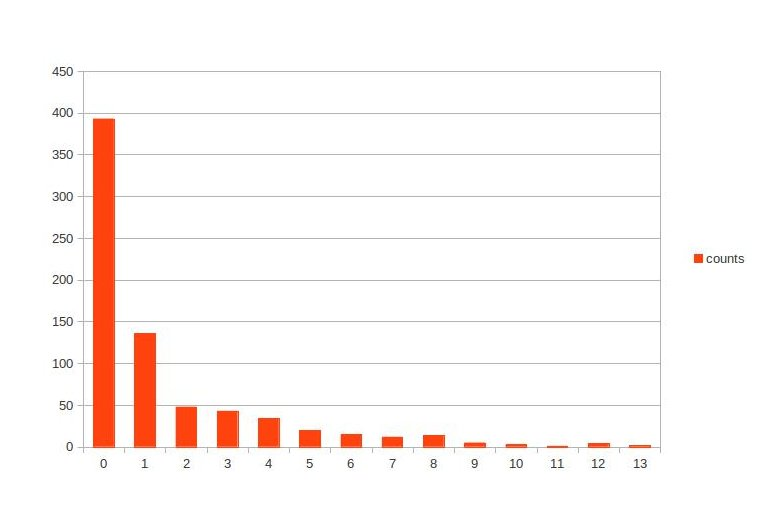
\includegraphics[scale=0.6]{length_based_results_better.jpg}
    \end {center}
    \item word differences:
    \begin{itemize}
        \item \textbf{393} chunks had \textbf{0} difference in words
        \item \textbf{136} chunks where different by \textbf{1} word (missing or additional)
        \item \textbf{48} different by \textbf{2} words
        \item \textbf{56} with a difference over \textbf{5} words
    \end{itemize}
\end{itemize}

\newpage
For \textbf{503} speeches, with a pause longer than \textbf{300ms}:
\begin{itemize}
    \item time differences: \newline
    \begin{itemize}
        \item there were \textbf{154} chunks which time frame were within a \textbf{0.5s} difference, 
        \item average time difference was \textbf{5.24s}
        \item standard deviation was \textbf{5.23s}
        \item maximum time difference was \textbf{37.9s}
    \end{itemize}
    \begin{center}
        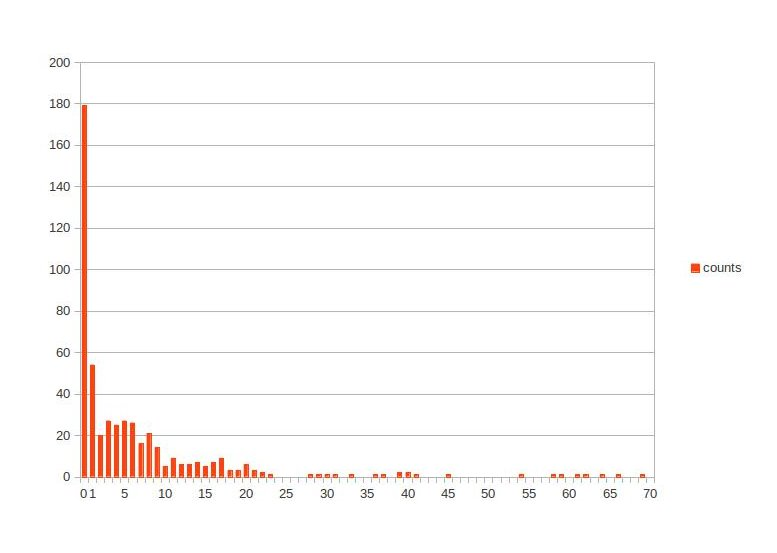
\includegraphics[scale=0.6]{length_based_results_worse.jpg}
    \end {center}
    \item word differences:
    \begin{itemize}
        \item \textbf{179} chunks had \textbf{0} difference in words
        \item \textbf{54} chunks where different by \textbf{1} word (missing or additional)
        \item \textbf{20} different by \textbf{2} words
        \item \textbf{56} with a difference over \textbf{10} words
    \end{itemize}
\end{itemize}

\newpage
\subsection{Conclusions}

The time statistics are showing a bit worse results, because word labels are more precise than chunk time frames. \newline

The results are within expectations, after all it is very crude algorithm. It probably could be improved though, however it is hard without introducing much more knowledge about language and possibly some additional training data (i.e. time of phonemes). \newline

This algorithm is a bit sensitive to a chunks created. If only the longer pauses are allowed, by increasing the holes filling factor from 200ms to 300ms in  speech detection algorithm, the results were considerably worse. \newline
In this case detected speeches contained more silence frames and consequently the total time is different, and the estimated times might be a bit more wrong. Another reason why it produces worse results might be related to the fact, that it also causes the speeches to be on average longer. This kind of random variables follow a rule, that they differ from an estimated value by square root factor, ergo longer parts, worse estimations.

\newpage
\begin{center}
    \section{Audio based alignment}
\end {center}
\subsection{Speech recognition}

Audio based alignment is simplified problem of speech recognition. Usually in speech recognition the language consist of millions of words in different conjugations, which may create many different sentences. In audio alignment we expect only one text and only one sentence at the time. \newline

Usually speech recognition is based on trained Hidden Markov Models with Gaussian Phoneme models, although successful systems rarely rely on single state phoneme model. \newline
As I mentioned before (3.1) there are many different allophones of single phoneme. A variations are largely attributed to surrounding they are spoken in. For example in polish there are softening phonemes 'i' and 'j', that clearly change how preceding or succeeding phonemes are realized. At some contexts it may happen that certain phoneme will lose it voice are even get silent completely, at another they will be strengthened with additional voice, i.e.: 
\begin{description}
	\item[“staw płytki”] $\rightarrow$ “w” loses it voice and starts to remind a phoneme “f”
	\item[“plac budowy”] $\rightarrow$ “c” gains additional voice and reminds a phoneme “dz”
\end{description}
And almost never one can cleanly separate two consecutive phones. \newline

 In order to better model different realisations of phonemes, an audio modelling contains models of phonemes at different triphone contexts. 
For every possible neighbourhood a given phoneme might appear, a separate Gaussian model is trained, for example a WSJ model from sphinx database contains 40 different phonemes and additional silence phoneme, that gives 68921 different triphones, however WSJ model contains over 110k elements,  because of additional information about location within a word. \newline

It is not over yet, because transitioning from phoneme to phoneme should be modelled somehow as well. The obvious solution is to train a triple state HMM, which will better fit the changing phone. \newline
That triples number of states. \newline

This huge number of different models requires a lot of training data, which is on one hand not easy to come along with, on another requires a lot of time to train with. \newline
Training data for speech recognition is one constant problem, which have to be dealt with. The problem is amplified, by the fact, that training samples should be small and very well described. That hardly can be done manually. \newline
Another bad news is, that a model trained on news feeds, is expected to perform poorly as a spoken address recognition software. \newline

\newpage

Once we have our audio model, than speech recognition is an easy piece, isn't it? \newline
Not really, since so many possible and often similar words make it a hard problem. Rarely a speech recognition software is based solely on audio model to recognize a sequence of phonemes. \newline
Problem is, that the number of states is too huge in order to be processed exhaustively, even though we can use a Viterbi algorithm to find a best (most probable) sequence of states for given observation sequence and we keep results only for a present moment in time (a single frame), that still gives a huge number
of kept states with calculated score. \newline

The sphinx library deals with this problem by searching in a breadth first search manner (meaning that it will keep states only from a current moment) and to cut on number of states to process, a priority queue is used, which keeps only best scoring ones. \newline

And this is the part of recognition software we would like to use for the alignment problem. \newline
The difference from here is that, we do know what the text is spoken, while for recognition there is no such knowledge. \newline
However let's dwell on this a little bit longer, so we can see what a huge simplification it makes. \newline

Let's start with a simple example by using WSJ dictionary: \newline
phoneme sequence “W AH N”, which  on it's own can be recognized as word “one” or “won” is also a prefix for 36 another different words and subsequence of total 117 different words. \newline
There is a sequence “W AH N S EH L F”, which assigned to word “oneself”, however it may also be from the end of word “penguin” (“W AH N”) and beginning of word “cellphone” (“S EH L F”). \newline

Sphinx library provides two ways of language modelling to tackle sucha ambiguity:
\begin{itemize}
    \item ngrams frequencies
    \item language grammar
\end{itemize}

For simple languages, like a sequence of digits or language containing one long sequence (like in case of text alignment), it is advisable to use language grammar. \newline
For general recognition software like Apple Siri, ngrams are necessary, although I am not convinced that they haven't used a sort of grammar for typical queries. \newline

Ngrams (in wsj n is maximum 3) are a way to assign a probability to word sequences. In above example it is expected, that “oneself” is more probable to occur in real word, than the later case, although obviously we can't judge so easily, since the probability of choosing these particular word depends on a probability of whole sentence. \newline

Anyway I think that's enough about speech recognition. \newline
For our purposes we need “only” audio model and word to phoneme sequence dictionary, in order to efficiently  align text to speech. \newline

\newpage
\subsection{Differences between english, russian and polish phonetics}

The sets of phonemes for any language differ slightly between publications and they differ even more between different audio models. For that reason I'm not going to introduce here established phonology for any language, however I'll try to match a phoneme set used by WSJ model for English, VoxForge model for Russian, Corpora and mine for Polish. \newline

In the table below I collected phonemes from four used sets and analysed differences, that may cause problem to represent some words using given phonetics and in result may cause problems with alignment. The table is organized so the similar phonemes are next to each other. If there is not alternative in a language, than the row remains empty. \newline

\newcommand{\strutA}[1]{% no space before strut
\rule[0pt]{0pt}{#1}% put text approx mid strut
}


\fontsize{10pt}{12pt}\selectfont
\begin{center}
\begin{tabularx}{\linewidth}{| p{1cm} | p{1.2cm} | p{1cm} | p{1.1cm} | p{1.1cm} | p{1cm} | p{1.1cm} | p{4.9cm} |}
\hline
\rowcolor[gray]{0.8}
English & example & Russian & example & Corpora Polish & Polish used by me & example & Notes on similarities
\\ \hline

AA & ad\underline{o}pt & a & \underline{а}рен\underline{а} & a & a & dwa &
\multirow{3}{\linewidth}{The most different from this set is English „AE”, which also shows a similarity to Polish and Russian „e”} \strutA{2ex}
\\ \cline{1-7}
AE & \underline{a}ct & aa & \underline{а}кт &&&&  \strutA{2ex}
\\ \cline{1-7}
AH & \underline{a}cute &&&&&& \strutA{2ex}
\\ \hline
AW & all\underline{ow} &&& a\_ (ą) && tą & \multirow{2}{\linewidth}{There is no such a vowel in Russian however it can be substituted with „oo l”, similar for my Polish model with „o ł”}  \strutA{4ex}
\\ \cline{1-7}
OW & aer\underline{o} &&&&&& \strutA{4ex}
\\ \hline
AY & b\underline{i}ke &&&&&& Simulated with Russian and Polish „a j”
\\ \hline
B & \underline{b}ill & b & \underline{б}ыл & b & b & \underline{b}yć & Quite similar
\\ \hline
&& bb & де\underline{б}ет &&&& A softened version of „b”, a bit different, but Polish and English „b”  can also be slightly softened
\\ \hline
&& c & \underline{ц}вет & c & c & \underline{c}oś & In English it is something like \newline „T S”
\\ \hline
CH & jackovi\underline{ch} & ch & дево\underline{ч}ка & ci (ć) & ć & czci\underline{ć} & 
\multirow{2}{\linewidth}{English „CH” is actually used for slavian words containing „c”, „ć”, „cz” like phonemes. Russian „ch” is similar to softened Polish „cz”, so it has to replace both „ć” and „cz”} \strutA{6ex}
\\ \cline{1-7}
&&&& cz & cz & \underline{cz}ego & \strutA{7ex}
\\ \hline
JH & \underline{j}ust &  &  & drz &  & \underline{dż}em & Simulated by „d zh” or „d ż”, English „JH” is quite similar.
\\ \hline
 &  &  &  & dzi (dź) &  & ka\underline{dź} & Simulated by „d zh” or „d ź”, English „JH” must simulate this one as well, although it also can be softened, it is not very similar.
\\ \hline
D & \underline{d}a\underline{d} & d & \underline{д}лина & d & d & \underline{d}uży & \multirow{2}{\linewidth}{Except for Russian and Polish „d”, all are a bit different. „dd” is again a softened version.}  \strutA{1ex}
\\ \cline{1-7}
 &  & dd & \underline{д}итя &  &  & & \strutA{1ex}
\\ \hline
DH & \underline{th}ey &  &  &  &  &  & No counterparts, something between „d” and „z”.
\\ \hline
\end{tabularx}
\end{center}

\newpage

\begin{center}
\begin{tabularx}{\linewidth}{| p{1cm} | p{1.2cm} | p{1cm} | p{1.1cm} | p{1.1cm} | p{1cm} | p{1.1cm} | p{4.9cm} |}
\hline
\rowcolor[gray]{0.8}
English & example & Russian & example & Corpora Polish & Polish used by me & example & Notes on similarities
\\ \hline
 &  &  &  & e\_ (ę) &  & s\underline{ę}k & Like „ee l” or „e ł” or „EH W”
\\ \hline
EH & thr\underline{ea}d & e & диван\underline{е} & e & e & \underline{e}la & \multirow{2}{\linewidth}{Similary as „a” alternatives, all sound quite alike, but a bit different. Russian differs in a stress, English „ER” is an "e" merged with a silent „r”} \strutA{5ex}
\\ \cline{1-7}
ER & thrill\underline{er} & ee & дн\underline{е} &  &  &  & \strutA{5ex}
\\ \hline
EY & thursd\underline{ay} &  &  &  &  &  & Like „e j”.
\\ \hline
F & \underline{f}ilm & f & \underline{ф}азы & f & f & \underline{f}ilm & \multirow{2}{\linewidth}{Very alike, except of course a softened Russian version}
\\ \cline{1-7}
&& ff & \underline{ф}илат &&&& 
\\ \hline
G & ea\underline{g}er & g & дол\underline{г}о & g & g & \underline{g}ęś & \multirow{2}{\linewidth}{As above}
\\ \cline{1-7}
&& gg & дол\underline{г}е &&&& 
\\ \hline
HH & \underline{wh}o & h & дома\underline{х} & h & h & \underline{ch}ata & \multirow{2}{\linewidth}{As above}
\\ \cline{1-7}
&& hh & ду\underline{х}и &&&& 
\\ \hline
IH & p\underline{i}cture & i & духам\underline{и} & i & i & \underline{i}gła & \multirow{2}{\linewidth}{Russian and English variations differ in stress, but all are quite similar} \strutA{2ex}
\\ \cline{1-7}
IY & acr\underline{ee} & ii & дух\underline{и} &  &  &  & \strutA{2ex}
\\ \hline
 &  & ae & ран\underline{я}т &  &  &  & This is a quite like „i” phoneme, but not completely. In Russian many vowels can be shortened to unrecognized version, which sounds like „i”.
\\ \hline
K & \underline{q}uote & k & \underline{к}афедр & k & k & \underline{k}to & \multirow{2}{\linewidth}{Very alike, except of course a softened Russian version.} \strutA{2ex}
\\ \cline{1-7}
 &  & kk & \underline{к}ефир &  &  &  & 
\\ \hline
Y & la\underline{wy}er & j & рано\underline{й} & j & j & \underline{j}ak & Very similar.
\\ \hline
L & \underline{l}awyer & ll & а\underline{л}екс & l & l & \underline{l}ato & Quite similar, although Russian is a softened version of „l”, so it doesn't cover all allophones of Polish „l”
\\ \hline
W & \underline{w}ork & l & \underline{л}ад & l\_ (ł) & ł & \underline{ł}ąka & Quite similar
\\ \hline
M & \underline{m}o\underline{m} & m & \underline{м}алы & m & m & \underline{m}a\underline{m}a & 
\multirow{2}{\linewidth}{Very alike, except of course a softened Russian version}
\\ \cline{1-7}
 &  & mm & малы\underline{м}и &  &  &  & 
\\ \hline
N & \underline{n}ail & n & \underline{н}адеюсь & n & n & \underline{n}os & Very alike.
\\ \hline
 &  & nn & наде\underline{нь} & ni (ń) & ń & ko\underline{ń} & No English alternatives, although it seems reasonable to use „N Y” sequence.
\\ \hline
NG & thi\underline{ng} &  &  &  &  &  & In Russian and Polish might be simulated with „n g” or just „n”, but no natural alternatives
\\ \hline
AO & f\underline{o}r & oo & подн\underline{ё}с & o & o & t\underline{o}k & Quite similar
\\ \hline
 &  & ay & п\underline{о}гадай &  &  &  & Non stressed version of „oo”, however it sounds more like „a”
\\ \hline
OY & foil &  &  &  &  &  & Can be simulated with „o i”.
\\ \hline
P & \underline{p}ack & p & \underline{п}оезд & p & p & \underline{p}as & 
\multirow{2}{\linewidth}{Similar. Russian allophones cover Polish and English phonemes.} \strutA{2ex}
\\ \cline{1-7}
 &  & pp & пом\underline{п}е &  &  &  & \strutA{2ex} 
\\ \hline
R & \underline{r}ace & r & \underline{р}ад & r & r & \underline{r}u\underline{r}a & \multirow{2}{\linewidth}{As above}
\\ \cline{1-7}
 &  & rr & \underline{р}юкзак &  &  &  & 
\\ \hline
S & \underline{s}and & s & \underline{с}цен & s & s & \underline{s}en &  \multirow{2}{\linewidth}{As above}
\\ \cline{1-7}
 &  & ss & \underline{с}егодня &  &  &  & 
\\ \hline
\end{tabularx}
\end{center}

\newpage

\begin{center}
\begin{tabularx}{\linewidth}{| p{1cm} | p{1.2cm} | p{1cm} | p{1.1cm} | p{1.1cm} | p{1cm} | p{1.1cm} | p{4.9cm} |}
\hline
\rowcolor[gray]{0.8}
English & example & Russian & example & Corpora Polish & Polish used by me & example & Notes on similarities
\\ \hline
SH & \underline{sh}op & sh & \underline{ш}ёлка & si & ś & \underline{ś}liwka & Quite alike.
\\ \hline
 &  &  &  & sz & sz & \underline{sz}osa & It is a bit similar to "ś", but no real alternatives.
\\ \hline
 &  & sch & \underline{щ}ека &  &  &  & No real counterpart. Can be simulated with „SH CH” and „ś ć' or „sz cz” and variations
\\ \hline
T & \underline{t}in & t & \underline{т}а & t & t & \underline{t}en & 
\multirow{2}{\linewidth}{Similar. Russian allophones cover Polish and English phonemes.} \strutA{2ex}
\\ \cline{1-7}
 &  & tt & \underline{т}ёмный &  &  &  & \strutA{2ex}
\\ \hline
TH & \underline{th}anks &  &  &  &  &  & No counterparts, something between „f” and „t”.
\\ \hline
UH & f\underline{oo}t & u & ёлк\underline{у} & u & u & \underline{ó}semka &
\multirow{3}{\linewidth}{All are quite alike, although subtle differences remain.}
\\ \cline{1-7}
UW & f\underline{oo}l & ur & \underline{ю}г &  &  &  & 
\\ \cline{1-7}
 &  & uu & абсол\underline{ю}т &  &  &  & 
\\ \hline
V & \underline{v}isit & v & \underline{в}аза & w & w & \underline{w}iedza &
\multirow{2}{\linewidth}{Similar. Russian allophones cover Polish and English phonemes.} \strutA{2ex}
\\ \cline{1-7}
 &  & vv & жи\underline{вь}ем &  &  &  & \strutA{2ex} 
\\ \hline
 &  & y & жив\underline{ы} & y & y & d\underline{y}m &
\multirow{2}{\linewidth}{Russian allophones differ in stress, but there is a problem with English equivalent. The most alike phoneme is „IH”.} \strutA{4ex}
\\ \cline{1-7}
 &  & yy & жив\underline{ы}х &  &  &  & \strutA{4ex} 
\\ \hline
Z & vi\underline{s}or & z & ва\underline{з}а & z & z & \underline{z}ebra & Quite alike.
\\ \hline
 &  & zz & ва\underline{з}е & zi (ź) & ź & \underline{ź}le & Russian and Polish are very alike. No English equivalent, „ZH” is the closest.
\\ \hline
ZH & vi\underline{s}ual & zh & \underline{ж}аба & rz (ż) & ż & \underline{rz}eka & Quite alike.
\\ \hline
\end{tabularx}
\end{center}
\fontsize{12pt}{14pt}\selectfont

I can try to draw some conclusions from the table alone. \newline

In English there are no natural alternatives in 8 cases, while in Russian only in 2 cases, although there are some other dissimilarities, it is clearly visible now (if it wasn't before), that Russian is much more similar language to Polish, than English. \newline
It might be a surprise though, that English isn't so different, and it seems possible to emulate every Polish word with English phonemes.
Maybe not too surprising though, after all we are all humans.

\newpage
\subsection{Grapheme to phoneme conversion grammar}

For the purpose of speech recognition we require very accurate dictionaries, that keep track of actual pronunciation of words with all possible variations. \newline

Usually the dictionaries are created by analysing actual recordings. \newline
I would like to propose a way of converting grapheme sequences into phonetic description, which might be good enough for many real life applications, like word alignment or even phoneme alignment. \newline
Nevertheless it would still be applicable only to problems which are easier than speech recognition, but only because it is a hard problem, which tries to get as much accuracy from sub-problems as it is only possible. \newline

Take a look at English  word “one” and “tone”. The differ with character, but a phonectics are: “W AH N”  and “T OW N”.  \newline
It doesn't seem to be trivial, and actually it might be necessary to study in more detail a language to find quite accurate grammar. However for Polish it might be easy enough to create such a grammar, that will give us enough accuracy to perform alignment task. \newline

We need at least three of such a grammars, converting to English, Russian and Polish phonemes. \newline
 Here are example conversions:

\begin{center}
\begin{tabular}{| p{3.5cm} | p{3.5cm} | p{3.5cm} | p{3.3cm} |}
\hline
\rowcolor[gray]{0.8}
Character sequence & English phoneme sequence & Russian phoneme sequence & Polish phoneme sequence
\\ \hline
a & AA & aa & a
\\ \hline
ą & AW & oo l & o ł
\\ \hline
b & B & b & b
\\ \hline
c & T S & c & c
\\ \hline
ci & CH IH & ch ii & ć i
\\ \hline
cia & CH Y AA & ch aa & ć j a 
\\ \hline
trz & T SH & t sh & t sz
\\ \hline
dż & JH & d zh & d ż
\\ \hline
dź & JH & d zh & d ź
\\ \hline
ch & HH & h & h
\\ \hline
h & HH & h & h
\\ \hline
ij & IY & --- & ---
\\ \hline
ó & UH & u & u
\\ \hline
rz & ZH & zh & ż
\\ \hline
ł & W & l & ł
\\ \hline
dzia & JH Y AA & d zz aa & d ź j a
\\ \hline
ź & ZH & zh & ź
\\ \hline
ś & SH & sh & ś
\\ \hline
\end{tabular}
\end{center}

\newpage

The conversion table looks similar to description of lexer tokens and in general it is what we do here. We convert word into tokens standing for a phoneme sequence. It might be a good idea to use regular expression in the grammar, however I haven't found a need for these, hence my rules convert a character sequence only. \newline

My rules were able to produce a set of possible phoneme representations, simply by adding a set of phoneme sequences to the right side of the rule. These however didn't prove to be quite beneficial, and after a short time experimenting with it, I reduced number of sets dramatically. After awhile I actually used a different variants only for the word alignment and only when I used sphinx with foreign audio model. \newline


The algorithm looks as follows:
\begin{itemize}
    \item variables:
    \begin{itemize}
        \item $\bold{S}$ - a set of all rules in the grammar
        \item $\bold{P}$ - a set of potential candidates
        \item $\bold{c}$ - longest matched candidate so far
        \item $\bold{R}$ - output set of phoneme sequences
    \end{itemize}
    \item at the start we have:
    \begin{itemize}
        \item $P = S$
        \item $c$ is unset
    \end{itemize}
    \item iterate over a character sequence,
    \begin{itemize}
        \item remove all candidates from $P$, that will never be a match after adding current character,
        \item if exists such $p \in P$, that it is currently matched, set $c$ with $p$
        \item if $P$ is empty
        \begin{itemize}
            \item for each $s$ phoneme sequence in $c$:
            \begin{itemize}
                \item create $R_s$ by adding $s$ to each element of $R$
            \end{itemize}
            \item set new output $R = \cup_s R_s$ 
            \item new set of potential candidates is $P=S$
            \item move iteration pointer to the end of matched sequence $c$ 
        \end{itemize}
    \end{itemize}

\end{itemize}

I would leave here an open question if it is possible to create such a grammar for more accurate dictionaries.It might be, since phonemes are the effect of how comfortable it is to say a given sequence of phones and people are not really able to remember too complex conversion. It might be possible, that the grammar would need take into account some rare oddities, like word “one”, but there is definitely a finite number of such. In order to find such a grammar, probably a study on existing and trained dictionaries should be done, but this is out of the scope of this project.

\newpage
\subsection{Audio model alignment and results.}

This part is relatively easy, because sphinx library already support word alignment using any audio model. It requires only a phonetic dictionary, which we can create using conversion grammar from previous chapter.  Whole conversion works similar to recognizing word, the same breadth first search algorithm with queue of best results is used, except that a HMM for whole language is created from simple grammar, which allows only one big sequence of words. \newline

We would like to test word alignment using English (WSJ) model and Russian (VoxForge) and compare it to some manually aligned sample. \newline

For my testing recording I used a 5 minute and 20 seconds of audiobook “Doktor Piotr” by Stefan Żeromski and 16 minutes and 20 seconds of audiobook “Boże Narodzenie” by Maria Dąbrowska. \newline
They were aligned by two different, but generally normal people (no experts) with purpose to make alignment as accurately as possible without selecting too much or too little. However while the person aligning “Doktor Piotr” considered overlapping to be forbidden, the person aligning “Boże Narodzenie” didn't have this presumption. This small fact changes statistics a bit especially for smaller time differences. \newline

Another difference between those texts, is that I have never seen any mistake in text for “Doktor Piotr”, at least in those first 5 minutes, but I've seen wrong words in the “Boże Narodzenie”, where the reader has replaced them with something different, or the text was incorrect, nevertheless there are some discrepancies. \newline

\newpage

With English model I haven't got too much luck. The problem with the algorithm for word alignment is that once it goes wrong, then it never goes back on track again. With English model after \textbf{38} seconds of “Doktor Piotr” it incorrectly assigned 3 seconds to word “części” after \textbf{62} words and it never recovered. For “Boże Narodzenie” it has gone wrong after \textbf{257} seconds on word “czarownicach” after \textbf{503} words. \newline

The statistics for “Boże Narodzenie” however shows, that before it goes bad it actually aligns first \textbf{503} words quite nicely:
\begin{itemize}
    \item Maximum difference (start or end): 			\textbf{0.559s}
    \item Maximum difference (start or end), if label was to short at one end: 			\textbf{0.559s}
    \item Average difference  (start or end):			\textbf{0.032s}
    \item Error counts depending on time thresholds:
    \begin{center}
        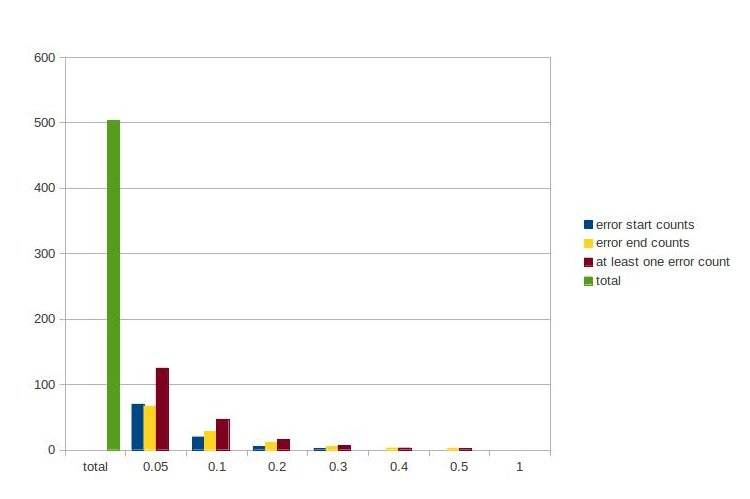
\includegraphics[scale=0.6]{boze_narodzenie_word_english_results.jpg}
    \end{center}
\end{itemize}

It seems that there weren't any substantial errors in the matching, although apparently the English audio model has some trouble with phoneme “cz”, which I'll remind was replaced by English “T SH”, which sounds more softened, than actual pronunciation. It is hard to figure out some other way of representing this one, and even though it looks like it could be used, some more elaborate method should be invented. Usually when word goes bad, the algorithm assigns too long selection to it, so maybe checking the time if it goes wrong and the to try some kind of recovery? I think it is possible, but I haven't explored this in more details. \newline

\newpage

I also tried Russian model, which haven't got problems as above and I could have generate statistics for whole alignment: \newline

The “Boże Narodzenie” statistics are:
\begin{itemize}
    \item Total number of words:				\textbf{1779}
    \item Maximum difference (start or end): 			\textbf{2.451s}
    \item Maximum difference (start or end), if label was to short at one end: 			\textbf{0.543s}
    \item Average difference  (start or end):			\textbf{0.016s}
\end{itemize}
The error counts regarding different time thresholds:
\begin{center}
    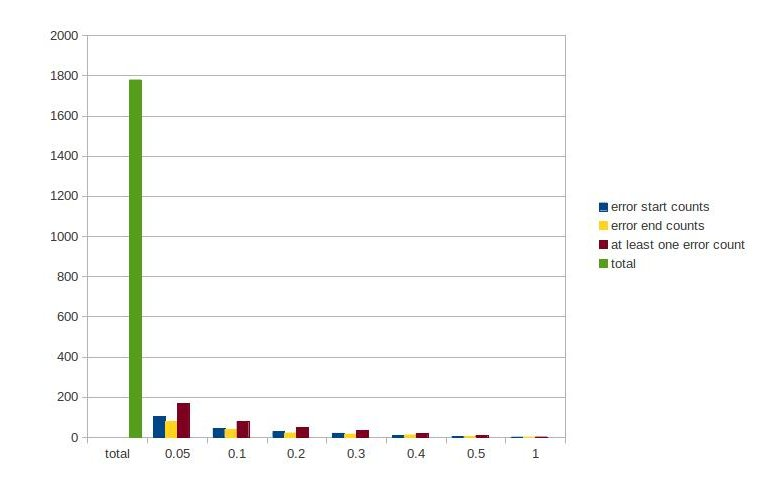
\includegraphics[scale=0.7]{boze_narodzenie_word_russian_results.jpg}
\end{center}

\newpage

The statistics for “Doktor Piotr” sample are:
\begin{itemize}
    \item Total number of words				\textbf{585}
    \item Maximum difference (start or end): 			\textbf{1.354s}
    \item Maximum difference (start or end), if label was to short at one end: 			\textbf{0.534s}
    \item Average difference  (start or end):			\textbf{0.033s}
\end{itemize}

The error counts regarding different time thresholds:
\begin{center}
    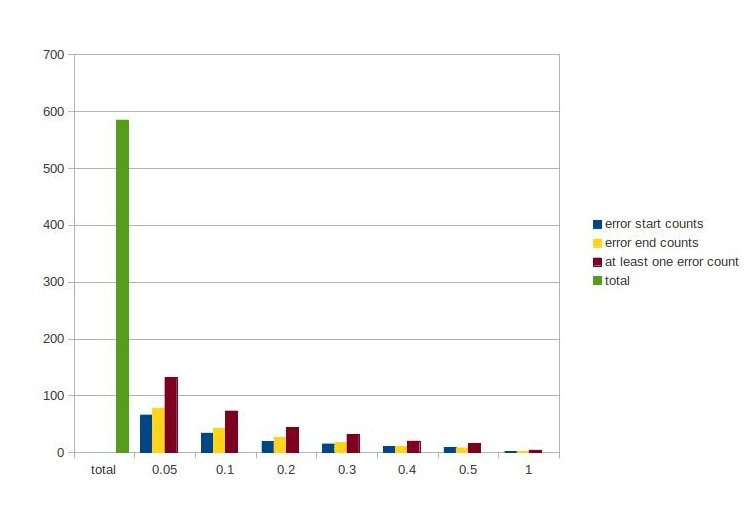
\includegraphics[scale=0.7]{doktor_piotr_word_russian_results.jpg}
\end{center}

\newpage
Analysing the above statistics it can be noticed, that even if English model didn't go wrong, it still seems to perform worse, than Russian model. The average difference is twice bigger than for the former.  Also the counts of errors in relation to total number of aligned words shows, that Russian models outperforms the English one, what is quite understandable, since we knew apriori, that Russian is much more similar to Polish. \newline

It is also noticeable, that they perform a bit differently. While English model finds borders of the word quite well, except for spectacular failures of course, the Russian on other hand frequently happens to include a pause after the word. This is a bit problematic for many different applications, except maybe for training, which can deal with that. Anyway since for English, the algorithm failed to finish the alignment, it may have happened, that it would show similar behaviour in later parts of the book. \newline

The additional pause added to a word label isn't completely bad, since it means, that we are quite sure, that given selection contains an assigned word, and that there is very little total misses. Direct observation of collected data supported that conclusion. There were very few total misses and only related to alignment conjunctives (“w” especially).\newline
From autopsy of collected data we also see, that the biggest mismatches were committed, when accounting a silence as a part of word. \newline

One could try to further improve above method, at least by meddling with a phoneme conversions or maybe even training dictionary from a corpus, to get a better phoneme representation. I can't be sure at this point how big impact has the simple conversion grammar on results, although it doesn't seem to be the most promising room for improvement. \newline

My final conclusion is that, regardless of some mismatches, it is a quite nice method for word alignment, especially for the purpose of further improvements in speech recognition systems and audio model trainings. 

\newpage
\begin{center}
    \section{Phoneme alignment}
\end {center}
\setcounter{equation}{0}

\subsection{Using foreign audio model}

I would like to use a trained Russian audio model (VoxForge) to align a selection of audio stream for each phoneme. \newline
Having aligned words, I would like to do it per word basis. \newline

Audio model is a trained Hidden Markov Model for each phoneme in a context of neighbouring phonemes or for all occurences of the phoneme with no context. Each HMM contains three states with transition table and probabilities of each transition as well as a set of normal distribution at each state, to calculate emission probability of observations (audio frames). \newline
By merging together phoneme models we get a HMM for whole input text. Of course before first we need convert this text to sequence of phonemes and then to sequence of HMMs, but this can be acchieve similarly as in chapter 5. \newline

Having HMM we can calculate the best possible sequence of states (using Viterbi algorithm) and all audio frames assigned to states from a single phoneme HMM should form together a single allophone of the phoneme. After that it just matter of calculating initial and ending time for each such a phone to produce an alignment. \newline

In my experiments I tried to do exactly this, however I've noticed that:
\begin{itemize}
    \item firstly, a transition score is absolutely meaningless for the alignment problem,
    \item secondly, only main phoneme is really important, and enter and exit state only produce a noise, which doesn't help substantially in solving my problem. It might be because, the model was Russian and it wasn't well fit for Polish speech.
\end{itemize}
In the end my algorithm used only main state without any transition probabilities. \newline

The Gaussian distributions were extracted using sphinx library in a form of SenomeScorer objects, which is able to calculate score for given observation. A best sequence was found using a Viterbi like dynamic programming algorithm, which was all too similar to many other DP algorithms in this project. \newline

At each iteration I processed a single audio frame.\newline
The entry data for iteration $k+1$ is a partial solution array $R_k$. At the index $i$ in array $R_k$ a score of most probable seqeunce of $i$ states observing $k$ audio frame is stored. The output of$k+1$-th is $R_{k+1}$. \newline 

The next values of solution array $R$ are calculated from a formula:
\begin{equation}
    R_{k+1, i} = argmax_j (R_j + \sigma_i(k+1))
\end{equation}
where $\sigma_i(k+1)$ is a log likelihood of emitting $k+1$-th audio frame by state $i$. \newline
This is a general Viterbi algorithm, but in my case there were only two outgoing states for each state in a HMM, so actual formula is:
\begin{equation}
    R_{k+1, i} = max(R_{i-1}, R_{i}) + \sigma_i(k+1)
\end{equation}

\newpage
This algorithm can be used with any scorers, so let's try to train the Gaussian distributions ourselves.

\subsection{Training phoneme distribution using word alignment}

Again I assume, that I already have word alignment (from chapter 5) and I would like to use it as my input training data. The data have very nice granularity,
and i.e. the sphinx training software can use a data, which is larger then that, although it is advised, that it will be small and accurately described (i.e including information silences). \newline
From chapter 5 we could see, that my data was not as accurately described, since the initial word alignment can be wrong by including in a selection quite long pauses, which my algorithm can't know about in advance. \newline

Training algorithm is a variation of EM algorithm and consists two steps:
\begin{itemize}
    \item \textbf{expectation step} – alignment of phonemes given previously trained distribution and using an algorithm from 6.1 for each word separately
    \item \textbf{maximization step} – calculating normal distribution for each phoneme from assigned observations obtained by expectation step
\end{itemize}

Phoneme representation of a given word was once again created using our conversion grammar with a small twist, that this time I'm not going to use Russian ones, but a set of Polish phonemes, refined in a series of experiments and described in chapter 5. \newline
In order to tackle with a problem of unexpected pauses, a silence phoneme (“sil”) was added at the beginning and at the end of each word phoneme sequence. \newline

Initial distributions are calculated from an initial simple selection of phoneme observations. For each word, it's phoneme sequence $\{p_1, ..., p_k\}$ and aligned audio sequence $\{f_1, ..., f_n\}$, a frame $f_j$ was assigned to phoneme $p_i$ if and only if $ (i - 1) \frac n k < j <= i \frac n k$.\newline

A total likelihood is calculated. When it converges below given threshold, then algorithm terminates and phoneme models are saved. \newline

Note that, the alignment algorithm has a complexity of $\Theta(nm)$, where $n$ is a number of states and $m$ is the number of audio frames. The size of the chunks we want to align or more important the number of phonemes in a given chunk, has a great impact on the total time of execution. Extracting words might really improve the time of audio model training for any variation of above method.

\newpage
\subsection{Results}

Tests are performed using Corpora corpus, which contains audio recordings of digits, names and some unusual sentences for tens of different speakers. \newline
My testing speech is created by merging all the files in random order for one speaker. The phoneme alignment is prepared by changing times of the labels from the recording put in $i$-th place by a total time of all recordings from first $i-1$ places. \newline

Merged recording contains a 7 minutes and 26 second of audio data, a total of \textbf{843} spoken words and \textbf{3611} phoneme labels. \newline
The Corpora phonetics differ a bit from what I used in Polish model and definitely differs from Russian phonemes. In order to compare the alingments the I had to convert phonemes to the same set. Most of the time it was relatively easy and I just converted a Corpora phoneme to the one used by me. However there were certain cases where it was not easy.\newline
A sample of needed changes: \newline
\begin{itemize}
    \item in my Polish models after soften consonant (like “nie”) I added additional “j” phoneme (resulting with “ń j e”) and Corpora didn't always have anything there, \newline
    the additional phoneme was ignored in the matching
    \item similarly in Russian conversion I never added additional phoneme (resulting with “nn e”), and Corpora sometimes had “i” phoneme in similar situations, \newline
    as above the additional phoneme was ignored
    \item Corpora used actual phonetics replacing soften versions of i.e. “z”, “zh” with alternatives (“s”, “sz”) and vice-versa (hardening), \newline
    the phonemes were considered similar and were matched against each other
    \item Corpora had separate phoneme for “ą”, “ę”, “dz”, “dż” like and I always split them into more phonemes, \newline
    the phonemes were merged into one and the merged was matched against testing label
    \item Corpora used a “?” symbol to indicate unrecognizable phonemes, which I actually found out from other recordings, \newline
    this one was replace with appropriate phonemes
    \item in one case few phonemes were merged into one shortened version, as speaker joined two words into one, \newline
    as above it was replaced with real phonemes and matched against
\newpage
\end{itemize}
Resulting matching was checked manually after the changes. \newline

Each matched phoneme had starting and ending time. Statistics produced about matching times agreement include an average start and end time difference, a maximum time difference and number of pairs of labels where time frame agreed with a certain error.

\newpage
Phoneme alignment using Russian audio model. \newline
A resulting match contained \textbf{3570} of pairs.
\begin{center}
    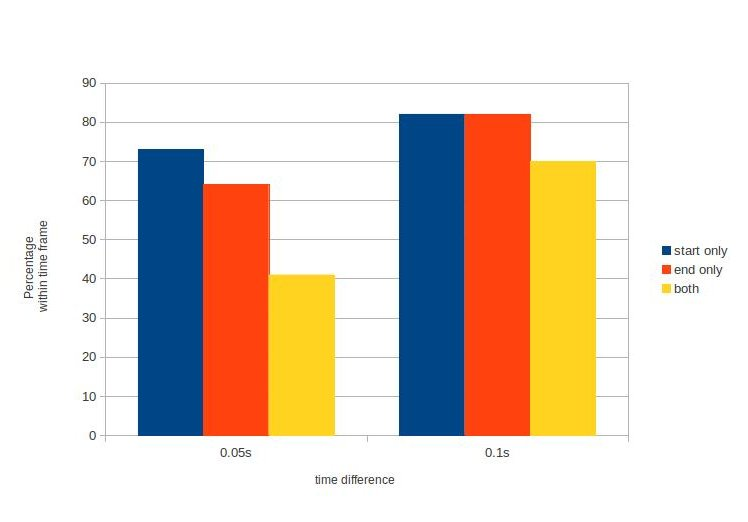
\includegraphics[scale=0.4]{corpora_phoneme_russian_results.jpg}
\end{center}
\begin{center}
    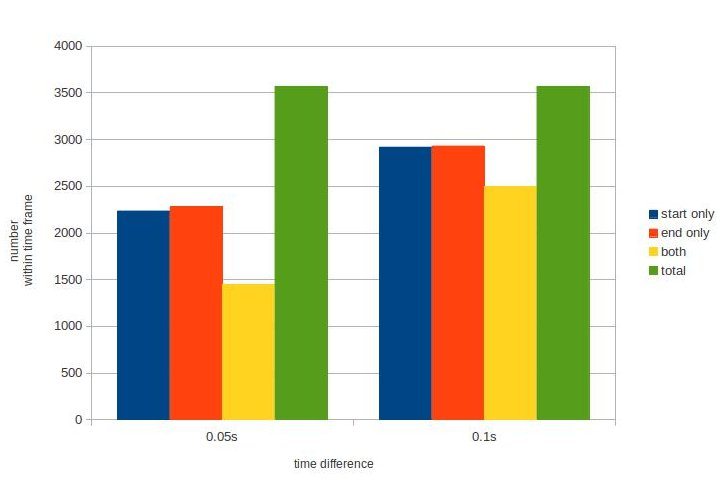
\includegraphics[scale=0.4]{corpora_phoneme_russian_counts.jpg}
\end{center}

\begin{itemize}
    \item Average start difference: \textbf{ 0.0571s}
    \item Average end difference: \textbf{0.0574s}
    \item Maximum time difference:\textbf{0.516s}
\end{itemize}

The results are not perfect at least, however one can see, that maximum time difference is around half a second, which at least tell us, that word alignment is with quite a nice accuracy. \newline
It was hard to expect anything better, after all the actual phonetics are different yet there was still a nice alignment for nearly 70\% of phonemes.

\newpage

Statistics for phoneme alignment using trained Gaussian models from aligned words.
A matching phonemes contained \textbf{3611} pairs.
\begin{center}
    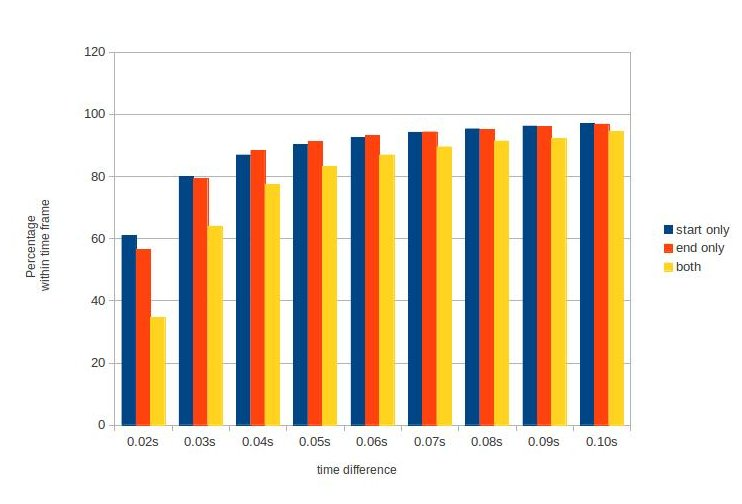
\includegraphics[scale=0.55]{corpora_phoneme_trained_results.jpg}
\end{center}
\begin{center}
    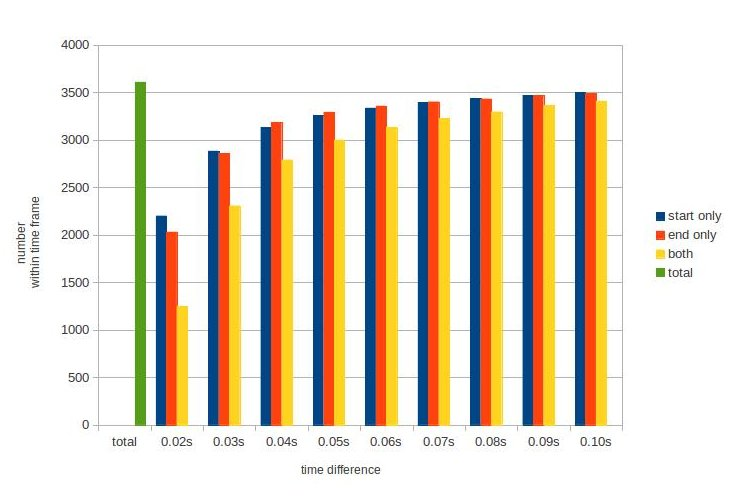
\includegraphics[scale=0.55]{corpora_phoneme_trained_counts.jpg}
\end{center}
\begin{itemize}
    \item Average start difference: \textbf{0.02402s}
    \item Average end difference: \textbf{0.02439s}
    \item Maximum time difference:\textbf{0.5131s}
\end{itemize}

\newpage

The average difference is down by 58\% and while using Russian audio model only 40\% of pairs agreed on both ends with a 0.05 second of error, a trained model could agree on 83\% of pairs, while getting to 95\% within an error of 0.1 second. \newline

Strangely the maximum stayed the same, what actually can indicate, that the word alignment, done using Russian audio model, might be a culprit here. \newline

Considering the fact, that we haven't use a specifically trained audio model for Polish language and we didn't have any knowledge of actual phoneme representation, then results are really good, although probably when using a better trained model, the percentages might be much better. \newline
Actually according to [28], it is possible to obtain a phoneme alignment within error of 0.02s with accuracy over 90\%. I am not near this, but consider this method as an entry point for more elaborate training and aligning methods. \newline
The important thing to remember is, that it was possible using only Russian audio model and conversion grammar, which contained only 158 rules. 

\newpage
\begin{center}
    \section{Training audio from large audio files}
\end {center}
\setcounter{equation}{0}

In this chapter I'll try to answer a question if it is possible to use audio recordings, that are 20 minutes to several hours long, with only exact recored text of the speech and yet being able to train a model from a given audio, that would be good enough for text alignment purposes, if only for recordings of very good quality, like audio books. \newline \newline

\subsection{Using imperfect large chunk alignment as a training database}

In the chapter 4 I described a method, that finds larger chunks of speech and matches parts of text to them, based on punctuation marks and pauses. As we have seen in the results, the output was quite inaccurate, however around 54\% of the chunks had been correctly identified, and around another 25\% had been nearly correct (less than 3 words difference). That doesn't seem to be good enough, but maybe we could train a model from it anyway. \newline

First of all as I mentioned before, training audio model from a large chunks requires quite a lot of time, because of complexity $\Theta(nm)$, where $n$ is a number of phonemes and $m$ is the size of audio chunk, what is more or less quadratic in relation to a number of characters in a chunk. \newline
Secondly we would expect, that longer streams might reduce our chance for a proper convergence of phonemes, but maybe not nearly as much as incorrectly assigned ones. \newline

Because of that I chose only chunks, that are shorter than a given constime time threshold. This value is problematic to choose automatically, because shorter texts, may require to use all of them in order to be able to train good enough model.For the longer texts may it may be enough to use only a few seconds short ones.
In any case a certain amount of training data is required. It is hard to believe, that it would be possible to train anything from a 10 second sentence. \newline

For the chosen chunks the algorithm converts assigned text to a phoneme sequence and between any two words additional silence phoneme is inserted, and at the beginning and at the end of the block. \newline
Once we do this, we have quite a similar set up as in chapter 6 when I wanted to train phoneme models having word alignment. At this point I haven't changed anything and the algorithm proceeds in the same manner. \newline
Just as before initial distributions are trained from the same crude assignment and as before the training uses a variation of EM algorithm, where estimation step is an alignment of phonemes and maximization step uses assigned frames to train the next generation of distributions. \newline

The only problem with this approach is, that the aligned chunks may be quite long (several tens of seconds) and this increases the runtime of the algorithm quite substantially, so a proper upper time threshold should be chosen. Anyway it is still a better way, than perforimg the task manually.


\newpage
\subsection{Word alignment with imperfect model}

This part has the closest resemblance to the speech recognition. Because we need to align a text that will be converted to many thousands of phonemes, it is infeasible to calculate a proper best sequence alignment. At each frame of audio, we would have to calculate a best sequence ending with each phoneme and since there are an order more frames than states, it would be just too many operations to complete the task in a reasonable time. \newline

I have visited this kind of problem before in chapter 5: an explosion of the number of states in speech recognition. The solution there was to cut on number of states by keeping a fixed size priority queue with a best scoring sequences only. In our case it should behave at least as well. \newline

The alignment is performed on a whole text at once. At first it is converted to a phoneme sequence $P = \{p_i, ..., p_n\}$, with additional “sil” phonemes at the beginning, at the end and between each two consecutive words. \newline

A state $s_i$ is a phoneme at given position $i$ in $P$ sequence and a normal distribution $N(\theta_{p_i})$,
and can be seen as a duple: $s_i = (p_i, N(\theta_{p_i}))$, where $\theta_{p_i}$ are parameters of normal distribution trained for a phoneme $p_i$. \newline
Each two states are $s_i \neq s_j \iff i \neq j$, although two phonemes and their models might be equal to each other. \newline

Queue at my algorithm contains a fixed number $N$ of best scoring sequences ending at $N$ states. \newline
In other words for each state $s_i$ at most one sequence is kept in a queue only and only if there are no more than $N-1$ states, for which best performing sequences ending at the states have worse score than a best score of all sequences ending at the state $s_i$. \newline
Even simpler my queue is a map with $N$ elements, where keys are states and values are sequences, which got the best score for a state being a key so far. \newline
Each sequence added to a queue may:
\begin{itemize}
    \item not be stored if all scores in map are greater than added sequence score
    \item may replace a value of the same state if previous sequence had worse score
    \item may be added as new element in the map, but if number of entries in a map is bigger than $N$, then a worse scoring sequence is removed with it's key (state)
\end{itemize}
This particular implementation performed noticeable better than the one, where I just remembered best scoring sequences regardless of ending state. \newline

The initial value in queue is an empty sequence ending with state $(p_1, N(\theta_{p_1}))$

\newpage

The algorithm iterates sequentially over frames in the audio stream. \newline
At the beginning of iteration $k+1$ we have a partial result of best scoring sequences in the queue, for the first $k$ frames. \newline
From a sequence $S$, its ending state $(s_i, N(\theta_{p_i}))$ and it's score $\phi_S$ two new sequences can be produced at iteration $k+1$. 
\begin{itemize}
    \item $S'$ with ending state $(s_i, N(\theta_{p_i}))$ and score $\phi_S + N(\theta_{p_i})(f_k)$
    \item $S''$ with ending state $(s_{i+1}, N(\theta_{p_{i+1}}))$ and score $\phi_S+N(\theta_{p_{i+1}})(f_k)$
\end{itemize}
For each sequence in queue produced by $k$-th iteration we create two new sequences as above and add them to a new queue, that will be a result of the current iteration. \newline

At the end of audio stream, we choose a best sequence, which then has to be converted into a phoneme alignment, which in the next phase has to be converted into a word alignment. \newline

Notice that it is highly unlikely that we will be having some sequences in the queue, that will be ending with a state that is far from a state that should be assigned to a current frame, or at least this is an idea behind the algorithm. Since all states from the queue have indexes greater than a certain $k$, it might be possible, that there exists a common prefix among all sequences in the queue. If this is the case, than it would be possible to convert this common prefix to word labels, even though we haven't processed whole stream. Since we will never change our mind about this prefix, then this action can be considered as a sentence recognition. \newline
Obviously in general speech recognition problem, we would have to add some additional probabilities of observing a given sequence of words into the algorithm, but the idea would be similar.

\newpage

\subsection{Results}
Let's see how word alignment performs bearing in mind results from chapter 5, where I used prepared audio models from other languages. \newline

The statistics for sample of “Doktor Piotr” are: \newline
\begin{itemize}
    \item Total number of words				\textbf{585}
    \item Maximum difference (start or end): 			\textbf{0.422s}
    \item Maximum difference (start or end), if label was to short at one end: 			\textbf{0.371s}
    \item Average difference  (start or end):			\textbf{0.044s}
\end{itemize}
The error counts regarding different time thresholds:
\begin{center}
    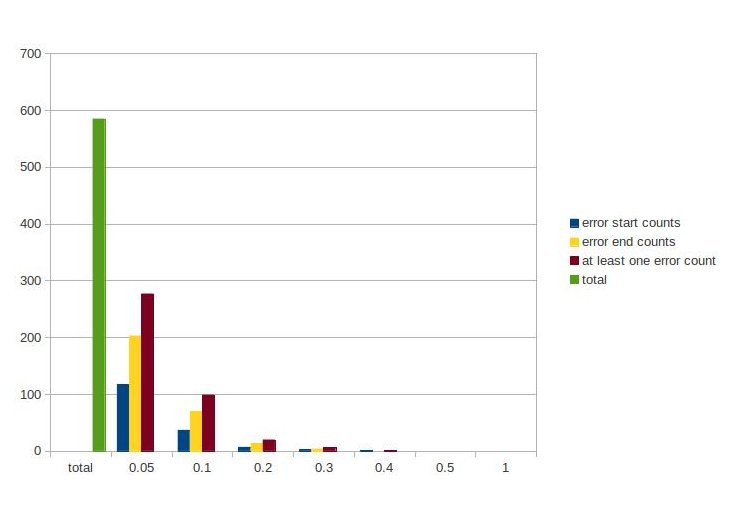
\includegraphics[scale=0.6]{doktor_piotr_length_based_counts.jpg}
\end{center}
Dropping to 0 at 0.5 second difference, while getting to 99\% of correct tags for error of 300ms.

\newpage
The “Boże Narodzenie” statistics are: \newline
\begin{itemize}
    \item Total number of words				\textbf{1779}
    \item Maximum difference (start or end): 			\textbf{0.606s}
    \item Maximum difference (start or end), if label was to short at one end: 			\textbf{0.605s}
    \item Average difference  (start or end):			\textbf{0.046s}
\end{itemize}
The error counts regarding different time thresholds:
\begin{center}
    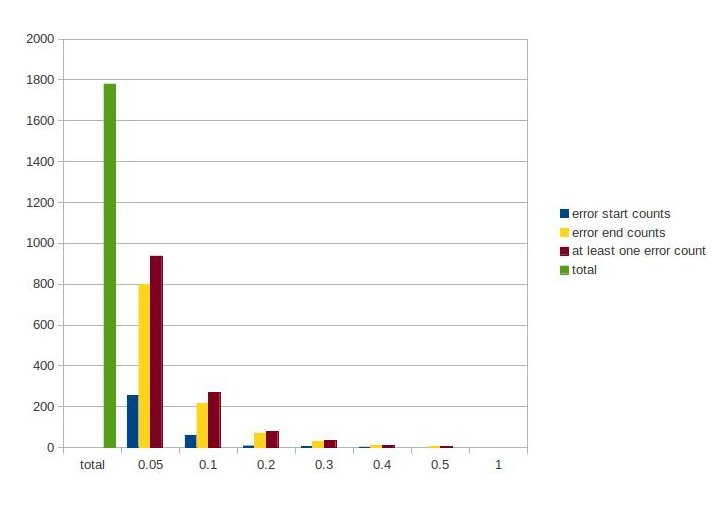
\includegraphics[scale=0.6]{boze_narodzenie_length_based_counts.jpg}
\end{center}
Dropping to 0 at 1 second difference, while exceeding 98\% of correct tags for error of 300ms.

\newpage
\subsection{Conclusions}

Firstly without diving into detailed analysis, the alignment without using any prepared audio model was able to align text with the word granularity and with a precision, that was not instinctively suspected. \newline
The best news is that, the algorithm was able to train quite accurate model for Polish language, for a single person with only 16 minutes of recording, that it could have been used to for alignment purposes. \newline

There are another good news, because it doesn't show a similar behaviour as alignment with Russian audio model, where the algorithm happened to assign quite long pauses to word labels.
It also seems, that the error counts drop much more quickly as the time of error threshold increases. It is hard to say how much the problem with silences impacts these difference, but one conclusion, that can be drawn for this, is that our alignment doesn't have too many total misses, although it may happen, that the algorithm frequently assigns too short part of the stream to words. \newline

The inspection of labellings shows, where the count of erroneous labels for small time thresholds comes from. It appears, that this approach does indeed suffer from an opposite problem to the one with extra silence parts. Apparently it often shortens ending of word labels. It is visible from count statistics as well, as a yellow bar indicating ends of word alignment is much higher than the red one for beginnings.
This is not good, although a small amendment, can be introduced to counter the effect, by adding a small constant time to the end of each label. \newline
The problem also showed in the average time difference, which is up to 3 times bigger than for alignment with Russian audio model. Let's not forget though, that these were trained from only 70 minutes long and 16 minutes long recordings, while the Russian one was trained from much larger database.

\newpage
\begin{center}
    \section{Testing alignment with synthesizer}
\end {center}
\setcounter{equation}{0}

What do we need phoneme alignment for? For training purposes it is not needed really, since a word or sentence level tagging is great enough. \newline
There is one application, that is widely used: from train announcements through automatic reading to  blind people support systems. It is a speech synthesizer, and such, that not only can be easily understood, but also sounds human alike. People tend to dislike artificial things that resemble humans to closely, but not completely. The automatic announcement systems can't be creepy or people will feel uneasy around it and may not want to hear it at all. Personally I hate synthesized audio books, which are just so unpleasant to listen to. \newline

It is nearly impossible to record all possible words at all possible forms to create well sounding synthesizer even for quite small announcement systems. An obvious alternative is to use a proper phoneme alignment to extract and combine parts from completely unrelated sentences, to produce a new form of or totally new word. \newline \newline

\subsection{Testing application of a synthesizer}

Except for uncountable possible applications of synthesizer, we can firstly use it as an additional way for testing our alignments, especially phoneme alignment. Dry statistics are not necessary the most intuitive way to check how our software performs and in the case of phonemes, it may actually be a much better testing ground. People don't agree too well what part of recording constitutes for a phoneme, if only because a single phone is barely perceivable by a human, so naturally such a manual alignment must escape to alternatives method of trying to find a part of word, which doesn't sound like it should. \newline
It is a similar technique to synthesizing words with an audio assigned to phonemes, but instead of doing this manually, we can try to this automatically. \newline

Testing is relatively straightforward and requires a good ear and a bit of time. We synthesize some sentences which may contain some of interesting phonemes and the we check if doesn't sound odd or if it is even understandable. 

\newpage
\subsection{Synthesizing speech with phoneme alignment}
Speech synthesizing can be simple and hard depending on what we actually want to get in the end and how much can we invest into preparation of audio files. \newline

On one end we have an easy problem of combining spoken words and phrases into sentences and the only thing we need to do, is match a silence part together. \newline
On the other we have a complete synthesizer, which don't have any prepared audio data and tries to produce the sound signal on it is own. It is doable, but currently all such a synthesizers have very little in common with a human speech and sound very robotic. Synthesizing a human like speech this way at this moment is completely outside our capabilities, but we can't disprove, that it won't be possible someday, after all in theory it is “only” a matter of simulating human respiration organs. \newline

Current top performing synthesizers are settling somewhere at the middle. Although for announcement system (i.e. in trains) it looks like it never synthesizes single word, but all are already recorded and it only combines them into larger statements. It might be feasible in this case, but most of the time it is impractical, because of the number of words needed to be recorded by a living, breathing and wanting to be paid human. Recording of million of words would take around 7 weeks of non-stop work assuming, that recording of one word would take only a second. And that is nearly not enough, especially for languages where conjugation is much more complex than in English. \newline

The solution is to use much smaller recording set and use it to create/synthesize words, that don't exist in the set. \newline

I experimented with two algorithms for word synthesizing. First is a bit better for testing purposes of phoneme alignment, while the second produces better results. Both algorithms used as an input audio recording tagged with phonemes. \newline


Both algorithms have a common part of choosing word candidates and merging them altogether. The only difference is a part of creating candidate when the word doesn't exist in the input text. \newline

In the common part we use a function, that scores a merging of two candidates $c_k$ and $c_{k+1}$ for $k$-th word and ($k+1$)-th word. \newline
The score is an euclidean difference between a small number of sequential frames from the ending of $c_k$ and the beginning of $c_{k+1}$. \newline
The beginning is a prefix of any $c_i$, which has a length not greater than a fixed fraction of $|c_i|$. \newline
Similarly the ending is a suffix of any $c_i$, which has a length not greater than the same fixed fraction of $c_i$. 

\newpage

Synthesizing algorithm:
\begin{enumerate}
    \item For each word in the text:
        \begin{enumerate}
            \item extract all parts of recording, that are tagged with the word
            \item if the extracted set is empty, then synthesize the word.
        \end{enumerate}
    \item Add between words a silence set, which are untagged parts of recording, \newline
          choose only the ones that satisfy durations constraints
    \item Choose a best sequence of audio streams using dynamic programming as below:
        \begin{enumerate}
            \item partial result array $R_0$ is initialized with $\{0\}$
            \item iterate over word sequence $\{w_1, ..., w_n\}$:
                \begin{enumerate}
                    \item entry data for $k+1$-th iteration is $R_k = \{s_1, ..., s_{|C_{w_k}|}\}$,
                    where $C_{w_k}$ is set of candidates for $k$-th word,
                    and $s_i$ is a score of best scoring merged stream ending with a $i$-th candidate
                    \item next score set $\{s_1', ..., s_{|C_{w_{k+1}}'|}\}$ is given by a formula:
                    \begin{equation}
                        s_i' = argmin_{j \in \{1,...,|C_{w_k}|\}} (s_j + score(j, i))
                    \end{equation}
                \end{enumerate}
            \item recreate best scoring sequence either from partial scores or with additional data stored in forward run
        \end{enumerate}
    \item Merge calculated sequence into one audio stream.
\end{enumerate}

\newpage

\subsubsection{Simple end to end synthesizer}

Actually this algorithm skips a little bit the part with synthesizing an audio stream for a given word.
The 1b part of above algorithms is changed to this:

\begin{enumerate}
\item
    \begin{enumerate}
        \setcounter{enumii}{1}
        \item if the extracted set is empty then:
        \begin{enumerate}
            \item convert word into sequence of phonemes
            \item for each phoneme
            \begin{enumerate}
                \item extract from the set of recordings parts, that are tagged with the phoneme
                \item add the set as a candidate set with phoneme as new word
            \end{enumerate}
        \end{enumerate}
    \end{enumerate}
\end{enumerate}

In the end a word, that was not found in the input text, is synthesized by combining extracted phoneme parts. \newline
It is calculated together with other words (or their phonemes) and it may not be optimal for each word, but whole sentence should sound ok. \newline
\newline

This algorithm is a bit better for checking correctness of phoneme alignment, because it combines phoneme signal end to end, so if something is wrong it should be immediately heard in the output stream. \newline
For the same reason it will have a poorer quality, because even if the aligner is perfect, the boundary frames might have some sound artefacts caused by preceding or succeeding phoneme, i.e. it is quite common, that the last vowel of the sentences changes to a breathing sound, when a speaker is exhaling or breathing in after longer sentence, and that is quite hard to separate, without actually training for recognizing breathing sounds, but to train them, you need a text with marked occurrences of such. \newline
\newline

The resulting audio contained quite some of such a artefacts and sometimes a bit additional silence here and there. The phonemes seemed to be more or less in order, but the word was a bit hard to understand, because the flow was kind of odd and very unnatural. Clearly it isn't a good synthesizer.

\newpage
\subsubsection{Middle to middle synthesizer}

In this algorithm each non-existing word was synthesized separately resulting with only one candidate for each word to be combined in the last phase of common part. \newline

The input to the algorithm is a phoneme alignment of the recording:
\begin{equation}
    L = \{ W_1, W_2, ..., W_n \}
\end{equation}
 where element $W_i$ is a phoneme sequence $\{p_{w_i, 1}, ..., p_{w_i, |w_i|}\}$ created from word $w_i$,
 accompanied with the assignment function $f$, that for each $p_{w_i, j}$ returns a unique (regarding pair for indexes $(w_i, j)$ and not actual phoneme) part of audio stream, i.e. $\{f_k, ..., f_{k+m}\}$. \newline

The algorithm first looks for candidates to be merged into a synthesized stream:
\begin{itemize}
    \item convert word to phoneme sequence $\{\rho_1, ..., \rho_n\}$
    \item for each $0 \leq i \leq n$ start with an empty set $S_i$:
    \begin{itemize}
        \item for each $W_k \in L$ and for each $0 \leq j \leq |w_k|$ find a maximum value of $m$, \newline
              where $j+m < |w_k|$ and $\forall_{z \in <j, j+m>} p_{w_k, z} = \rho_{i+z-j}$,
        \item if $m > 2$ add a sequence $\{p_{w_k, j}, ..., p_{w_k, j + m}\}$ to set $S_i$
    \end{itemize}
    \item if $S_i=\emptyset$, then repeat second step, but now add a sequence if $m>1$
\end{itemize}

An element $S_i$ from the sequence of candidate sets $\{S_1,...,S_n\}$ resulted from above procedure, has the property, that each of it's elements are a subsequences of phoneme representation of the synthesized word, and all of them start with a phoneme $\rho_i$. \newline

It is possible, that one of such a candidate set would be empty, if there were no such a subsequence, but it is not quite likely, that in larger file it will happen. In this case we could fall back to some variation of this method and the first one, but a preferred subsequences of length of at least 3 are quite common.\newline

The next part of algorithm has to choose which of them should be merged and at which frame they are to be combined. \newline
The algorithm once again uses a dynamic programming technique in quite similar manner to the common part, the main difference is in the scoring function.

\newpage

The algorithm iterates over the candidates $\{S_1, ..., S_n\}$. \newline
The k-th iteration processes the set $S_{k+1} = \{s_1, ..., s_l\}$. \newline
At the beginning of iteration ($k+1$)-th for each element $s_i \in S_k$ the algortithm keeps a best scoring synthesized stream, for which a phoneme representation ends with a sequence $s_i$. \newline

The next iteration results are obtained by calculating best scoring synthesized stream for each element $s_j' \in S_{k+1}$, as follows. \newline

A score between candidates $s_i$ and $s_j'$ is calculated by finding a closest frame (by Euclidean distance) of the second phoneme in $s_i$ and a first phoneme in $s_j'$, which should correspond to the same $\rho_{k+1}$. \newline

If the second phoneme from $s_i$ has assigned consecutive frames from $a$ to $b$: $\{f_a, ..., f_b\}$, \newline
and the first phoneme from $s_j$h as assigned frames from $c$ to $d$: $\{f_c, ..., f_d\}$, \newline
then a score of combining those two sequences is:
\begin{equation}
    argmax_{x \in <\frac {(a + b)} 2 - \frac {|a - b|} \delta, \frac {(a + b)} 2 + \frac {|a - b|} \delta>, y \in <\frac {(c + d)} 2 - \frac {|c - d|} \delta, \frac {(c + d)} 2 + \frac {|c - d|} \delta>}(dist(f_x, f_y))
\end{equation}
where $\delta$ is a constant chosen based on empirical experiments. \newline

A picture shows intervals from two sequences, for which a distance is calculated, and if a closest frames were chosen as the arrow indicates, how a resulting stream would look like:

\begin{minipage}[0,0]{15cm}
    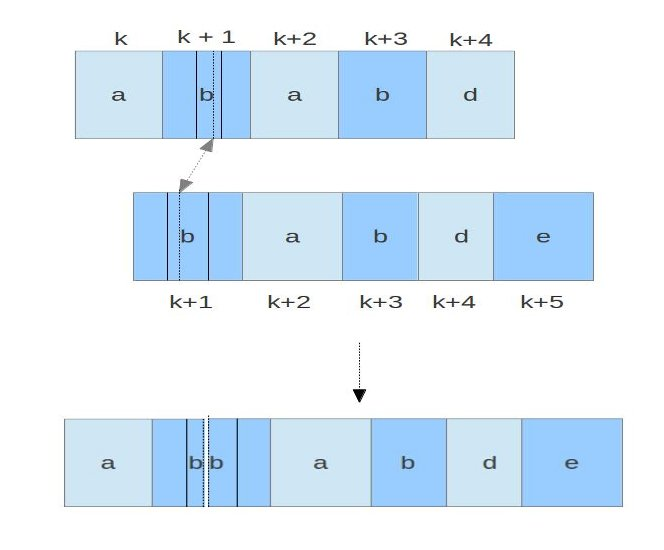
\includegraphics[scale=0.5]{audio_merging.jpg}
\end{minipage}
\begin{minipage}[15cm,0]{4cm}
$s_i$
\newline
\newline
\newline
\newline
\newline
\newline
$s_j'$
\newline
\newline
\newline
\newline
\newline
\newline
\newline
\newline
output 
\end{minipage}
At the end a best scoring stream is returned as a resulting synthesized audio for input word.

\newpage
\subsection{Results and conclusions}

How does it work? It is hard create automatic test for speech synthesizing. Theoretically I could rerun word alignment to see how it would perform for synthesized speech, however the alignment works even if there are occasional mismatches between text and speech, so it doesn't really gives much, except maybe checks if there are no total misses. It poses a certain challenge to create such a test, the challenge, that I'm not necessary willing to take, since I am a bit more optimistic about total misses, especially after looking at statistics from previous chapters and in the end, the human inspection is necessary anyway to check how it actually performs. \newline

My idea of test is to try to synthesize various texts more and less randomly chosen and see for myself how it performs and where it behaves incorrectly. \newline

A recording used for synthesizing is a full text of “Doktor Piotr” which contains an hour and 22 minutes of speech. The phonemes are aligned by training model from initial word alignment obtained using method from chapter 7, that doesn't need external audio model, but trains it itself using initially time and pause based alignment. \newline

I chose couple of unrelated texts, which contain some of tongue twisters, a part of epic poem “Pan Tadeusz”, a part of novel “Przedwiosnie”, and couple sentences from cultural column in “Politika” weekly magazine. \newline
\newline

The first algorithm shows quite substantial flaws in phoneme alignment. Apparently a lot of phonemes has additional trailing frames from a succeeding phoneme, what renders the created speech, to be incomprehensible, although closer inspection shows, that actual phonemes are correct, just not perfectly aligned. And it doesn't matter if the model was trained from the word labelling obtained using Russian audio model or Polish trained from initial pause based alignment. It shows, that an alignment with more perfection is needed for this kind algorithm. \newline

The second algorithm deals with this problem by combining phonemes middle to middle, so no ending is ever included. 


\begin{center}
\begin{tabular}{| p{8cm} | p{8cm} |}
\hline
\rowcolor[gray]{0.8}
synthesized texts &
Notes on erroneous parts in synthesized speech using words and phonemes initiated by pause based alignment
\\ \hline
"Rosja przedwojenna była wymarzoną areną dorobku dla ludzi tego typu zwłaszcza pochodzących z Królestwa" &
- „areną” – „a” is missing \newline
- jumps between phonemes are clearly visible, although they are not disturbing enough to cloud the meaning
\\ \hline
"Wiadomości zaczerpnięte w klasach gimnazjalnych wrodzona inteligencja która wraz ze zdrowiem towarzyszyła poszukiwaczowi posady i na zawołanie zjawiała się nie siana i nie pielęgnowana wytrzymałość odwaga wesołość i pewna odrobina drwiny z Moskala u którego się służy lecz nad którym jednak panuje się mimo wszystko torowały drogę od niższej do wyższej pozycji" &
- the phonemes of word „mimo” are quite short, so listener need to be really focused, to not miss a meaning of the word, \newline
- after „zjawiała się” there are two extra words „do wyjścia”,
closer inspections showed, that „się” was included as whole, but was badly aligned,
\\ \hline
"Trzeba przyznać że nie ostatnią rolę grała w tej operze protekcja cicha pokorna dobra wróżka prowadząca za rękę od niskiego do coraz wyższego rodaka tu i tam zaczepionego nogą lub łokciem na tej rosyjskiej drabinie" &
- „przyznać” - „ć” is actually „ź” \newline
- „tej” is something else \newline
- „protekcja” - hearable „w” before „t” \newline
- „spokojna” - something extra after „k” \newline
- „zaczepionego” - „z” is missing \newline
- „drabinie” - „ie” is missing \newline
\\ \hline
"Chrząszcz brzmi w trzcinie w Szczebrzeszynie W szczękach chrząszcza trzeszczy miąższ Czcza szczypawka czka w Szczecinie" &
- „brzmi” - „żm” phoneme sequence was not found in whole text so it was omitted in the synthesized audio, \newline
- „czcza” sounds like „cza”, \newline
- „Szczecinie” - „ie” missing
\\ \hline
"Chrząszcza szczudłem przechrzcił wąż Strząsa skrzydła z dżdżu A trzmiel w puszczy, tuż przy Pszczynie Straszny wszczyna szum" &
- „wąż” - „ą” is missing \newline
- „straszny” - „ny” is missing \newline
- „szum” - „m” is strange
\\ \hline
"Litwo Ojczyzno moja ty jesteś jak zdrowie Ile cię trzeba cenić ten tylko się dowie Kto cię stracił Dziś piękność twą w całej ozdobie Widzę i opisuję bo tęsknię po tobie" &
- „cenić” - „ć” is missing \newline
- „stracił” - extra „e” or even kind of „em” \newline
- „piękność” - very short „e” \newline
- „ozdobie” - first „o” is missing, second sounds like „ą” \newline
- „tobie” - short „e”
\\ \hline
"Panno święta co Jasnej bronisz Częstochowy I w Ostrej świecisz Bramie Ty co gród zamkowy Nowogródzki ochraniasz z jego wiernym ludem" &
- „świecisz” - „ś” sounds weird like "sz" through teeth, \newline
- „co” - hearable „t” at end, \newline
- „gród” - missing „g”, \newline
- „nowogródzki” - extra „na” at the beginnings and „dz” sounds like „jz”, \newline
- „ochraniasz” - first „o” is actually „w”, \newline
- „wiernym” - quite bad, at the beginning there is extra „pły”, and there is missing „r” making it completely unrecognizeable
\\ \hline
\end{tabular}
\end{center}

\newpage

\begin{center}
\begin{tabular}{| p{8cm} | p{8cm} |}
\hline
\cellcolor[gray]{0.8}
synthesized texts &
\cellcolor[gray]{0.8}
Notes on erroneous parts in synthesized speech using words and phonemes initiated by pause based alignment
\\ \hline
"Jak mnie dziecko do zdrowia powróciłaś cudem Gdy od płaczącej matki, pod Twoją opiekę Ofiarowany martwą podniosłem powiekę I zaraz mogłem pieszo do Twych świątyń progu Iść za wrócone życie podziękować Bogu Tak nas powrócisz cudem na Ojczyzny łono" &
- „mnie” - extra „u” at the beginning, \newline
- „ofiarowany” - first „o” sounds like „he”
\\ \hline
"Tymczasem przenoś moją duszę utęsknioną Do tych pagórków leśnych, do tych łąk zielonych Szeroko nad błękitnym Niemnem rozciągnionych" &
- „łąk” - extra short „a” at the beginning
\\ \hline
"Do tych pól malowanych zbożem rozmaitem Wyzłacanych pszenicą, posrebrzanych żytem Gdzie bursztynowy świerzop, gryka jak śnieg biała Gdzie panieńskim rumieńcem dzięcielina pała" &
- „do” - extra „łe” at the end, \newline
- „rozmaitem” - sounds like „smeitem”, \newline
- „gryka” - noticeable short „ł” at the end, \newline
- „panieńskim” - „ie” is short, \newline
- „rumieńcem” - a pause between „m” and „ie”
\\ \hline
"A wszystko przepasane jakby wstęgą miedzą Zieloną na niej z rzadka ciche grusze siedzą" &
- „wstęgą” - only „gą” is recognizeable
\\ \hline
"na stole z powyłamywanymi nogami leżą śliwki czereśnie pomarańcze i ogórki" &
- „leżą” - extra „na” up front, \newline
- „czereśnie” - missing „re”
\\ \hline
"W czasie suszy szosa sucha" &
\\ \hline
"Za górami za lasami znajduję się wysoka wieża strzeżona przez smoka" &
\\ \hline
"Maksymalistyczny egzystencjalny program Mrożka polegał właśnie na stawianiu świata pod znakiem zapytania w świetle jak najbardziej trzeźwych zarzutów o jego niewystarczalność" &
- „maksymalistyczny” - first „m” is actually an „s”, extra „lny” at the end, \newline
- „mrożka” - „first „m” is actually „z”, \newline
- „polegał” - extra short trailing „o”, \newline
- „o” - very short and faint
\\ \hline
"Mrożek jako krytyk cywilizacji widział w niej nadto przemoc mechanizm mielenia jednostek na proszek W rewolucjach brzydził go fetor mierzwy w jaką zmieniają się górnolotne czyste ideały" &
- „mechanizm”- sounds like „mechaniźmie”, because „z” is „ź”, \newline
- „jednostek” - short but loud extra „w” at the beginning, \newline
- „brzydził” - noticeable „g” between „y” and „dz”, \newline
- „fetor” - trailing „e”, \newline
- „ mierzwy” - missing „y”, \newline
- „jaką” - a bit distorted and unrecognizeable, \newline
- „ideały” - „i” is replaced by „u” and extra „j” between „e” and „a”
\\ \hline
\end{tabular}
\end{center}

\newpage

\begin{center}
\begin{tabular}{| p{8cm} | p{8cm} |}
\hline
\cellcolor[gray]{0.8}
synthesized texts &
\cellcolor[gray]{0.8}
Notes on erroneous parts in synthesized speech using words and phonemes initiated by pause based alignment
\\ \hline
"Pomimo języka groteski którym tak chętnie się posługiwał był przede wszystkim piewcą głębi sztuki jej ocalającego kontemplacyjnego wymiaru" &
- „pomimo” - some artefact in ending „o”, \newline
- „jej” - something extra at the beginning, \newline
- „ocalającego” - some „r” after „oca”

\\ \hline
"Przy czym nigdy głośno o tym nie mówił Jednocześnie sceptycznie i ostrożnie podchodził do kwestii wyobraźni widząc w niej zasadę kierującą ludzkimi poczynaniami a co z kolei skutkuje każdorazowo totalitarną eksterminacją" &
- „kwestii” - last „i” like „j”, \newline
- „wyobraźni” - missing „ob” changing the meaning of the word, \newline
- „totalitarną” - „ą” sounds like „ąu”

\\ \hline
\end{tabular}
\end{center}

Synthesizer results are showing us what kind of mistakes the phoneme aligner makes and what exactly the percentages presented in previous chapter mean. \newline
It appears, that the word alignment is not perfect and sometimes it is off by selecting too much, although it doesn't seem to happen too often. Much more common mistake is assigning too little to the word label, what results with missing phonemes, although this might be case on any word misalignment, where phoneme alignment just couldn't find correct tagging. \newline

The most obvious conclusion is that, this kind precision is not enough for the perfect speech creation, although only 3 words among the synthesized sentenced were actually not recognizable, and among them, there was one, where it actually changed it meaning. \newline

Not every error in above table is a result of misalignment, some are outcome of the compactness of conversion grammar or plainly because of incorrect phoneme conversion. After all there is no guarantee, that conversion will produce a correct phoneme description. \newline

Also the synthesizer is not perfect and could be improved in many various ways, especially by improving the score of combining two consecutive words/phones to consider the whole similarity, so there are no sudden changes in volume or timbre. The main purpose of the simple synthesizer here is to check how phoneme alignment works, so these improvements are a bit out of scope of this thesis. \newline

Generally the created speeches were comprehensible and the meaning could be grasped quite easily. The effect seems to agree with brought up statistics for word and phoneme alignment. It is ok, but not perfect.


\newpage
\begin{center}
    \section{Summary and conclusions}
\end {center}
\setcounter{equation}{0}

I believe that I managed to show in this thesis, that word alignment can be done without much apriori knowledge.
My algorithm was able to return a decent alignment for input audio file and recorded text with only knowledge about:
\begin{enumerate}
    \item punctuation marks and their relationship to pauses
    \item a bit of knowledge about relationship between graphemes and phonemes (conversions grammars)
    \item a human anatomy and capabilities, especially about speech frequency ranges
    \item assumption that the input text has a high accuracy
\end{enumerate}
It would require further studies, but I believe it is possible to even further reduce necessary knowledge.
\begin{description}
    \item[Ad.1] this relationship might be unimportant, if we had large enough database and that may mean only a couple of hours of recordings, \newline
    the length based alignment might be ok even with character by character matching, and that would mean, that it is possible to learn, that certain characters are actually punctuation marks (repeatedly are assigned to silences?)
    \item[Ad.2] using actual graphemes instead of my conversions reduces the accuracy of the models, but there is no reason why using only graphemes wouldn't be enough
    \item[Ad.3] this is almost definitely unnecessary, since the only reason I used it in the first place, was not because it increases the accuracy, but because it improves the performance, but working with bigger frequency set should be possible and some perfomance can be regained i.e. by measuring distance from normal distribution and by merging close frequencies
    \item[Ad.4] obviously there exists a certain threshold where it would be impossible to train anything, but even in the situation where we would have couple of recordings and many texts without knowing which are which, it might be possible to find a matching, but it seems like a hard problem
\end{description}

\newpage

The future work could focus on improving above algorithms and creating a system, that is able to align single text or a set of them with much higher accuracy.
Promising improvements include:
\begin{itemize}
    \item bimproving the above algorithm by rerunning speech alignement with imperfect model
    \item combining model from couple of separete texts
\end{itemize}
Also it might be interesting to study if it is possible to perform such a alignment in more noisy environments especially for songs and crowd recordings. \newline
Even more intersting if it can be done for recordings with poor quality, like phone calls etc. These might be extra hard not only because of poor signal quality, but also because people's diction in daily situation is not very good and the flow of the text shows a lot of irregularities with different interruptions (people interrupt each other, sometimes thay wait for other to get back, etc). \newline
These are quite hard situations even for well prepared systems. \newline

One application of such a system would be automatic training for any language recogniton software with very little human interference. Currently the top speech recognition software is being developed mainly for English, while hundreds of other languages attracts much less attention. Unless English will become the world's official language and all of people will be able to speak English with similar accent, the need for such system is quite obvious. \newline
If it would be possible to generate a speech recognition software easily for any language, then a majority of people wouldn't be excluded from using certain technologies (SIRI, GoogleGlasses, etc). \newline

I also believe that by studying how computers can gain certain knowledge may prove to be beneficial in understanding how people learn, and that is not only useful, but purely interesting. \newline
I haven't exhausted the topic even in a slightest, since it is just a part of larger question: how one can learn a language without external help. How human infants learn to talk, and how computers can mimick (or not) to learn language as well. \newline
I think, that answering this question with great detail, may improve our solutions for human-computer interactions and others. \newline
However many there are applications, a pure exploration is always enough reason to study a question. If it was asked, let's try answer it. \newline

Each of results brought up in this thesis and whole project with all mentioned algorithms are available for git checkouts from: \newline
https://github.com/Heappl/speechtextmatcher or \newline
https://bitbucket.org/Heappl/speechtextmatcher.

\newpage
\begin{center}
    \section{Bibliography}
\end {center}

\begin{thebibliography}{99}
\bibitem{englishDict} Houghton Mifflin Company. \emph{The American Heritage Dictionary of the English Language}, Fourth Edition, 2000.
\bibitem{albertiiAnatomy} Prof. W. Alberti. \emph{The anatomy and physiology of the ear and hearing.}
\bibitem{piconeFundamentals} Prof. Joseph Picone \emph{Fundamentals of speech recognition}
\bibitem{olsonMusic} Olson Harry F. (1967) \emph{Music, Physics and Engineering}
\bibitem{volkman} Stevens Stanly Smith, Volkman John, Newman Edwin B. (1937) \emph{A scale for the measurement of the psychological magnitude pitch Journal of the Acoustical Society of America}
\bibitem{douglasCommunication} Douglas O'Shaughnessy (1987) \emph{Speech communication: human and machine.}
\bibitem{zwicker} Zwicker E. (1961) \emph{Subdivision of the audible frequency range into critical bands.}
\bibitem{melCepstrum} H.P. Combrinck and E.C. Botha \emph{On The Mel-scaled Cepstrum}
\bibitem{welchFFT} Welch P. (1967) \emph{The use of fast Fourier Transform for the estimation of power spectra: A method based on time averaging over short, modified periodograms}
\bibitem{smithDigital} Steven W. Smith \emph{The scientist and engineer's guide to digital signal processing.}
\bibitem{} A. Pinsky \emph{Introduction to Fourier analysis and wavelets}
\bibitem{} B.P. Bogert, M. J. R. Healy, J. W. Tukey \emph{The Quefrency Alanysis of Time Series for Echoes: Cepstrum, Psuedo-Autocovariance, Cross-cepstrum and Saphe Cracking }
\bibitem{} Seyed Hamidreza Mohammadi, Hossein Sameti, Amirhossein Tavanaei, Ali Soltani-Farani \emph{Filter-bank design based on dependencies between frequency components and phonem characteristic}
\bibitem{} Dr. James Glass, prof. Victor Zue \emph{Automatic Speech Recognition} MIT course.
\bibitem{} Daniel Jurafsky, James H. Martin \emph{Speech and language processing}
\bibitem{} B. Plannerer \emph{An Introduction to Speech Recognition }
\bibitem{} Davis, Marmelstein (1980) \emph{Comparison of parametric representation of monosyllable word recognition in continously spoken sentences}
\bibitem{} Ahmed N., Natarjan T., Rao K.R. (1974) \emph{Discrete Cosine Transform}
\bibitem{} Syed Ali Khayam \emph{The Discrete Cosine Transform (DCT): Theory and Application} 
\bibitem{} Crystal David \emph{Linguistic}
\bibitem{} Chomsky N., Halle M. \emph{The sound pattern of English}
\bibitem{} Jagodziński G. \emph{Gramatyka języka polskiego.}
\bibitem{} J.L. Rodgers, W.A.Nicewander \emph{Thirteen ways to look at the correlation coefficient.}
\bibitem{} Jae Myung \emph{Tutorial on maximum likelihood estimation}
\bibitem{} Prof. A. Moore \emph{Clustering with Gaussian Mixtures}
\bibitem{} Jeff A. Bilmes \emph{A Gentle Tutorial of the EM Algorithm and its Application to Parameter Estimation for Gaussian Mixture and Hidden Markov Models}
\bibitem{} M. Karaś, M. Madejowa \emph{Słownik wymowy polskiej.}
\bibitem{} John-Paul Hosom \emph{Speaker-Independent Phoneme Alignment Using Transition- Dependent States}
\end{thebibliography}

\end{document}
